\documentclass[article]{jss}

%% -- LaTeX packages and custom commands ---------------------------------------

\usepackage{thumbpdf,lmodern}
\usepackage[usenames,dvipsnames]{xcolor}
\usepackage[textwidth=8em,textsize=small]{todonotes}
\usepackage{amsmath}
\usepackage{amssymb}
\usepackage{float}
\usepackage{subfig}
\usepackage[labelfont=bf]{caption}
%\usepackage[demo]{graphicx}
%% another package (only for this demo article)
\usepackage{framed}
%% new custom commands
\newcommand{\class}[1]{`\code{#1}'}
\newcommand{\fct}[1]{\code{#1()}}
\newcommand{\R}{\mathbb{R}}
\newcommand{\ee}{\mathbb{E}}
\newcommand{\de}{\mathrm{d}}
\newtheorem{definition}{Definition}[section]
%% For Sweave-based articles about R packages:
%% need no \usepackage{Sweave}



%% -- Article metainformation (author, title, ...) -----------------------------

%% - \author{} with primary affiliation
%% - \Plainauthor{} without affiliations
%% - Separate authors by \And or \AND (in \author) or by comma (in \Plainauthor).
%% - \AND starts a new line, \And does not.
\author{M. Mehdi Moradi\\University of Jaume I
    \And Edzer Pebesma\\University of M\"unster
    \And Jorge Mateu\\University of Jaume I}
\Plainauthor{Achim Zeileis, Second Author}

%% - \title{} in title case
%% - \Plaintitle{} without LaTeX markup (if any)
%% - \Shorttitle{} with LaTeX markup (if any), used as running title
\title{trajectories: Classes and Methods for Trajectory Data}
 \Plaintitle{trajectories: Classes and Methods for Trajectory Data}
\Shorttitle{trajectories: analysing movement data}

%% - \Abstract{} almost as usual
\Abstract{
   The package \pkg{trajectories} presents different classes and methods to handle and summarise trajectory data in \proglang{R}. It also provides model fitting to moving objects using time series modelling in the package \pkg{forecast}. Moreover, when dealing with a list of moving data that overlap in time, \pkg{trajectories} develops some statistical methodologies which provide users with some information about the behaviour of objects over time and with respect to each other. Using some methodologies for spatial point patterns, available in the package \pkg{spatstat}, we present an estimator for the intensity function of trajectory patterns which highlights the more visited streets, dense paths, etc. Based on second-order summary statistics for spatial point patterns, \pkg{trajectories} proposes a variability area which shows the variation of the type of interaction between moving objects over time. We also discuss the discrepancy between the estimated intensity and the expected intensity per area per time. Our methods are applied to a taxi trajectory data from Beijing, China.
}

%% - \Keywords{} with LaTeX markup, at least one required
%% - \Plainkeywords{} without LaTeX markup (if necessary)
%% - Should be comma-separated and in sentence case.
\Keywords{Chi-map, Distance, Intensity, \proglang{R}, Second-order characteristics, Spatio-Temporal,  Taxi Movements, Trajectory}
\Plainkeywords{JSS, style guide, comma-separated, not capitalized, R}

%% - \Address{} of at least one author
%% - May contain multiple affiliations for each author
%%   (in extra lines, separated by \emph{and}\\).
%% - May contain multiple authors for the same affiliation
%%   (in the same first line, separated by comma).
\Address{
M. Mehdi Moradi\\
Institute for New Imaging Technology\\
University of Jaume I\\
Avda. Sos Baynat, s/n\\
12071 Castellon, Spain\\
E-mail: \email{moradi@uji.es}\\

\emph{and}\\

Edzer Pebesma\\
Institute for Geoinformatics\\
University of M\"{u}nster\\
Weseler Strasse 253\\
48151 M\"{u}nster, Germany\\
E-mail: \email{edzer.pebesma@uni-muenster.de}\\
URL: \url{http://ifgi.uni-muenster.de/} \\ \\
52{\textdegree}North Initiative for Geospatial Open Source Software GmbH\\
Martin-Luther-King-Weg 24\\
48155 Muenster, Germany\\
URL: \url{http://www.52north.org/}\\

\emph{and}\\

Jorge Mateu\\
Department of Mathematics\\
University of Jaume I\\
Avda. Sos Baynat, s/n\\
12071 Castellon, Spain\\
E-mail: \email{mateu@uji.es}\\
URL: \url{https://www3.uji.es/~mateu}
}

\begin{document}


%% -- Introduction -------------------------------------------------------------
\section[Introduction]{Introduction}\label{sec:intro}
Modern data collection techniques allow tracking objects continuously. This means that we do not only know the current location of a moving object, but we also track the objects over time. A set of some tracks from different moving objects may be considered a trajectory pattern. Another example is that in which we record the location of a group of moving objects (e.g. cars, pedestrians, animals) within a regular/irregular time sequence. \cite{guting05} focused on moving objects databases and extended database technology to deal with moving objects. \cite{challa2011} presented an introduction to the field of object tracking and provided solid foundation to the collection of diverse algorithms developed by academics, scientific researchers and engineers. \cite{hanks15} proposed a continuous-time, discrete-space (CTDS) model for animal movement. \cite{russell16} introduced an approach that models dependent movement by augmenting a dynamic marginal movement model with a spatial point process interaction function within a weighted distribution framework. \cite{hooten17} presented a natural basis function approach to constructing appropriate covariance models for movement processes. There are already some \proglang{R} packages available in \href{https://cran.r-project.org}{CRAN Task View: Handling and Analyzing Spatio-Temporal Data} to handle moving objects. Most of them are focused on handling and analysing animal movements such as \pkg{adehabitatLT} \citep{calenge06}, \pkg{tripEstimation} \citep{sumner2009}, \pkg{argosfilter} \citep{argosf}, \pkg{V-Track} \citep{V-Track}, \pkg{animalTrack} \citep{animalTrack}, \pkg{BBMM} \citep{BBMM}, \pkg{bcpa} \citep{bcpa}, \pkg{BayesianAnimalTracker} \citep{BayesianAnimalTracker}, \pkg{TrackReconstruction} \citep{TrackReconstruction}, \pkg{mkde} \citep{mkde}, \pkg{SimilarityMeasures} \citep{SimilarityMeasures}, \pkg{smam} \citep{smam}, \pkg{trip}\citep{trip}, \pkg{moveHMM} \citep{moveHMM}, \pkg{FLightR} \citep{FLightR}. In particular, the package \pkg{adehabitatLT} \citep{calenge06} provides tools to simulate trajectories using a Brownian motion, correlated Random walks and Levy walks. \cite{SimilarityMeasures} presented four different similarity measures in \pkg{SimilarityMeasures}. \cite{moveHMM} in \pkg{moveHMM} provided animal movement modelling using hidden Markov models. Using multiple regression, \pkg{fishmove} \citep{fishmove}  provides functions to predict fish movement parameters. R package \pkg{trackR} \citep{frick} provides infrastructure for running and cycling Data.

However, to the best of our knowledge, \proglang{R} is still missing a complete set of generic data structures and methods to effectively analyse trajectories without being limited to a particular domain. Figure \ref{taxitracks} shows routes passed by 5 different taxis on the 4th of Feb 2008 in Beijing, China. Each taxi has a different start/end time.
To avoid having a complicated plot, we have only displayed 5 tracks; the entire dataset will be analysed in Section \ref{sec:explo}.

Studying the behaviour of moving objects over time and their interaction, either between objects or with environment, plays a crucial role in understanding how they use space and more importantly how they interact each other. Moving objects are moving within a particular area over time, thus a snapshot of a trajectory pattern might be seen as a spatial point pattern. This aspect then empowers us to study the behaviour of moving objects within space and over time. A set of locations, usually non-uniformly distributed within a certain region, can be considered as a realisation of a spatial point process. Analysis of spatial point processes has been widely discussed in the literature \citep{MW03,IPSS08,D13,BRT15}. The \proglang{R} package \pkg{spatstat} \citep{baddeley05,BRT15} provides different tools for statistical analysis, model-fitting, simulation and tests on spatial point patterns. \cite{D13} has broadly considered the details of spatio-temporal point processes. Application of such processes can be found in traffic management, geography, forestry, ecology, epidemiology, seismology, astronomy and criminology. 

This paper describes a collection of tools provided by the \proglang{R} package \pkg{trajectories} to handle, simulate and statistically analyse movement data regardless of the domain, converting a trajectory pattern into a list of point patterns based on regular timestamps. We here propose different functions to analyse the behaviour of objects over time and how they use space and also how they interact with each other. The type of interaction between objects may vary over time. The effect of the environment on the type of interaction might also be of interest. Therefore, using the literature of spatial point processes, the \proglang{R} package \pkg{trajectories} opens up a new way of thinking about trajectory datasets. We define different classes to handle trajectories, and different functions for simulating and performing exploratory data analysis. We also borrow first and second-order characteristics from the literature of spatial point processes and, by adapting them to trajectory patterns, we aim at highlighting the most frequently used routes within the studied area together with disclosing the type of interaction between the objects over time. Moreover, the \pkg{trajectories} package fits time series models to the spatial coordinates of a trajectory dataset.

\begin{figure}[!h]
\centering
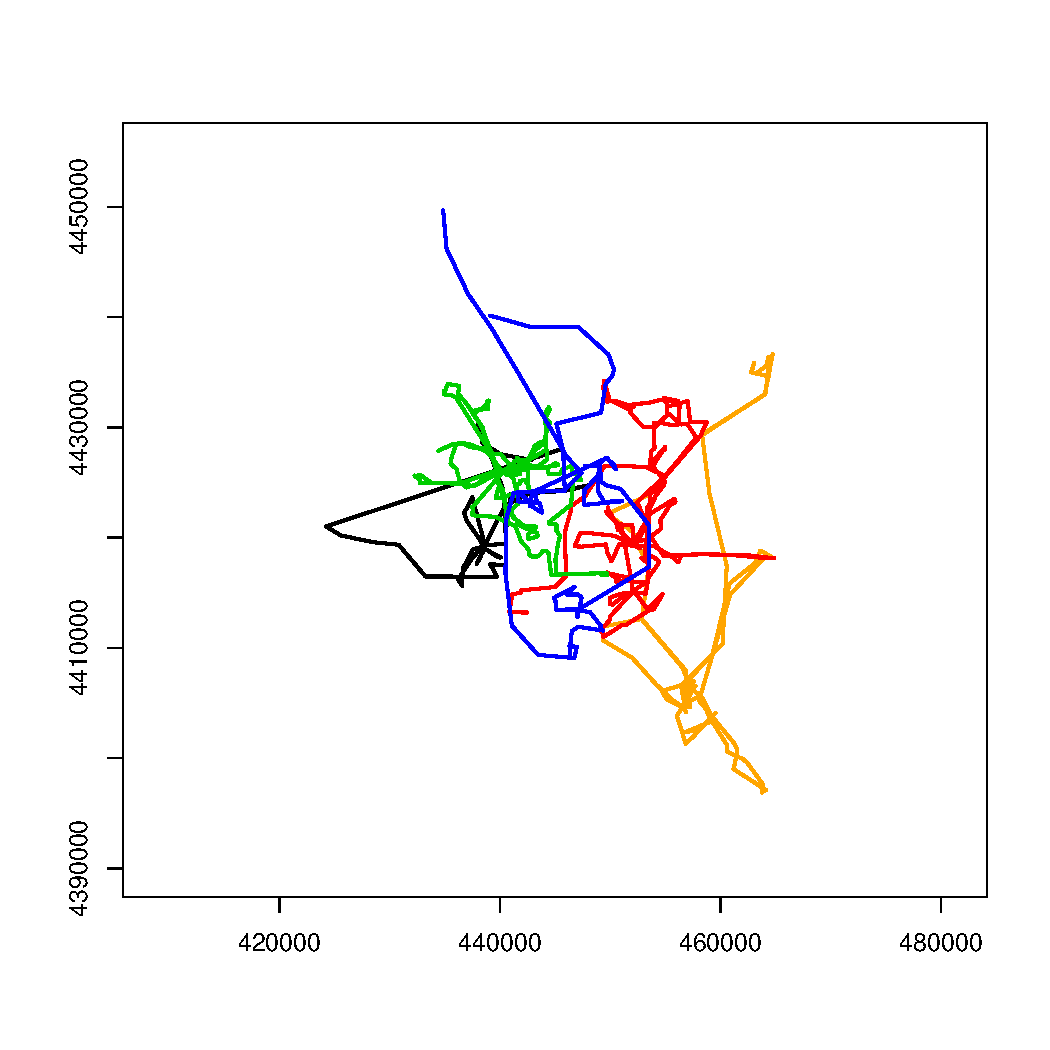
\includegraphics[width=0.6\linewidth]{Tracks-ex.pdf}
\caption{Trajectory pattern containing tracks of five taxis on the 4th of Feb 2008 in Beijing, China. Each color represents a different taxi track.}
\label{taxitracks}
\end{figure}

The plan of the paper is the following.
Section \ref{sec:setdef} presents some background and definitions.
Section \ref{sec:classes} describes different classes of trajectories and explains different methods to summarise trajectory data. Simulation and model fitting of trajectory data is described in Section \ref{simandfitt}. Section \ref{sec:explo} develops some statistical methods to perform exploratory data analysis and they are demonstrated through the taxi trajectory data from Beijing, China. The paper ends with some final conclusions in Section \ref{sec:summary}.

\section{Setup and definition}\label{sec:setdef}
Spatial point locations are usually analysed through spatial point processes, see \citep{MW03,daley07,BRT15}. Such events might also be labelled with the temporal instant, demanding then a spatio-temporal analysis \citep{D13}. Let $X$ be a spatial point process in $\mathbb{R}^2$ with intensity function $\lambda(\cdot) >0$ and second-moment intensity $\lambda^2(\cdot,\cdot)$. For any Borel-measurable real function $f(x)$ where $\int_{\R^2} |f(u)|\lambda(u) \de u < \infty$, it is satisfied
\begin{eqnarray}\label{campbell}
\ee \left[\sum\limits_{x \in X} f(x)\right]=\int_{\R^2} f(u)\lambda(u) \de u, \hspace{1cm} u \in \R^2.
\end{eqnarray}
Equation \eqref{campbell} has been broadly used in the literature of spatial point processes and it is called \textit{Campbell's formula}. Generally speaking, $\lambda(\cdot) $ is the expected number of points per unit area. Recall that if $\lambda$ is constant then $X$ is homogeneous, otherwise $X$ is called an inhomogeneous point process. One of the first and an important step in studying point processes is to investigate the intensity function. Estimating the intensity function of spatial point processes has been largely discussed \citep{D85,jones93,CSKWM13}. We denote a realisation of the point process $X$ with $n$ points as $\mathbf{x}=\{x_1,x_2,\ldots,x_n \}$; note that $n$ is not fixed in advance. 
In point process analysis, we only consider a single realisation of the underlying point process, and then analyse the behaviour of that realisation. However, we might be able to collect the location of spatial events according to regular or irregular timestamps over time. We then have a series of points over time per single object which can be considered as a single ``\textit{Track}''. For instance,  recording the location of a taxi over particular times results in the route passed by that taxi. We here consider a \textit{trajectory pattern} as a point pattern which lives in $\R^2$ but moves over time. This allows us to adapt the point process statistical methodology into the literature of \textit{trajectory patterns}.
  \begin{definition}
A \textit{trajectory pattern} is a dataset which provides observed 
tracks $(s_i)$ of a set of moving objects such as cars, humans, etc over a finite time period $T$. We denote a trajectory pattern consisted by $n>0$ single tracks as $S=\{s_i: s_i \subset \R^2, \hspace{1mm} i=1,\ldots,n  \}$, that is a countable set of tracks. Each $s_i$ is itself a countable set of points, e.g. $s_i=\{x_1^{s_i},x_2^{s_i}.\cdots, x_{m_i}^{s_i} \}$ with $i=1,\cdots,n$ where each $s_i$ consists of $m_i<\infty$ points that are associated with an increasing set of time stamps $t_1,...,t_{m_i}$, $t_j > t_{j+1} \forall j$.
\end{definition}
  We point out that the length of each of the tracks $s_i$ is not necessarily the same for all tracks. In other words, they might have different start/end times. Each single track $s_i$ represents the movement of a moving object within a finite time/area. It is usually supposed that locations of a moving object are recorded in regular timestamps. However, if timestamps are not regular, one can still interpolate the locations in regular timestamps. Therefore, each single track in $S$ might be seen as a set of points corresponding to the considered timestamps. Discretising all tracks of $S$ according to regular timestamps results in a list of point patterns (one per each time) which enables us to consider a trajectory pattern as a point pattern which is changing over time. Therefore, using point pattern methodology, one can study the behaviour of moving objects over time. For instance, the spatially varying distribution of objects and the type of interaction between them over time can be of interest. Assume that the trajectory pattern $S$ is observed within the time period $T$, thus discretising $T$ into a time sequence $\{t_i: t_i \subset T, i=1,\ldots,k \quad \text{where} \quad t_i < t_j \quad \text{if} \quad i< j \}$ generates a collection of spatial point patterns, say, $\textbf{x}_1,\textbf{x}_2, \ldots, \textbf{x}_k$ $(k>1)$.  Details are provided in Section \ref{sec:explo}. Nevertheless, one may still consider $S$ as a point process on $\R^{2\otimes k}$, where $\R^{2\otimes k}$ means $\R^2 \times \cdots \times \R^2$ for $k$ times when the length of timestamps is $k$. We do not discuss this other approach here.

\section{Classes and methods} \label{sec:classes}
In this section, we review different classes of trajectories to handle movement data in \proglang{R}. These classes were initially defined in the \proglang{R} package \pkg{spacetime} \citep{spacetime}. Before moving into the details and start analysing trajectory patterns, we load the package with:

\begin{Schunk}
\begin{Sinput}
R> library(trajectories)
\end{Sinput}
\end{Schunk}

\subsection{Track}
The class \class{Track} represents a single track followed by a person, animal or an object. Instances of this class are meant to hold a series of consecutive location/timestamps that are not interrupted by another activity. The class contains five slots: @sp to store the spatial points, @time to store the corresponding time, @endtime to store the end time when having generalised line geometries with one value per attribute for a set of points (otherwise, defaults to the time defined in @time), @data to store the attributes (covariate information) and @connections to keep a record of attribute data between points (e.g., distance, duration, speed and direction). A Track object can be created out of an \class{STIDF} object as follows
\begin{Schunk}
\begin{Sinput}
R> set.seed(10)
R> t0 = as.POSIXct(as.Date("2013-09-30",tz="CET"))
R> x = c(7,6,5,5,4,3,3)
R> y = c(7,7,6,5,5,6,7)
R> n = length(x)
R> t = t0 + cumsum(runif(n) * 60)
R> crs = CRS("+proj=longlat +ellps=WGS84") # longlat
R> stidf = STIDF(SpatialPoints(cbind(x,y),crs), t, 
+                  data.frame(co2 = rnorm(n,mean = 10)))
R> A1 = Track(stidf)
R> A1
\end{Sinput}
\begin{Soutput}
An object of class Track 
7points 
bbox: 
  min max
x   3   7
y   5   7
Time period: [2013-09-30 02:00:30, 2013-09-30 02:02:31]
\end{Soutput}
\end{Schunk}
\begin{figure}[!h]
\begin{center}
\begin{Schunk}
\begin{Sinput}
R> plot(A1)
\end{Sinput}
\end{Schunk}
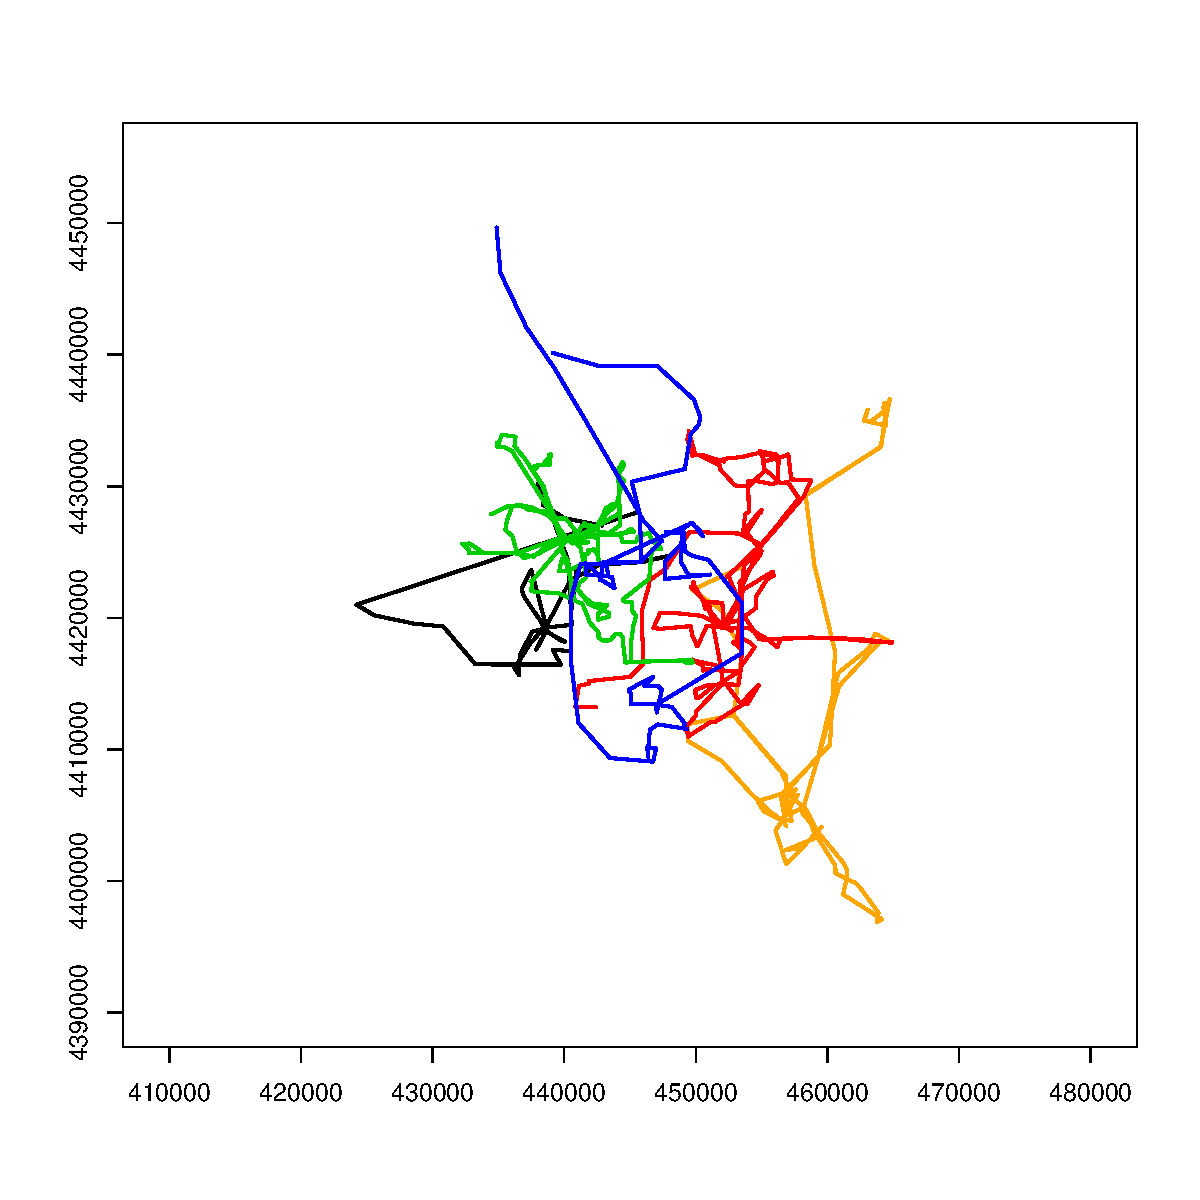
\includegraphics{article-004}
\end{center}
\caption{Single track A1 passed by person A.}
\label{figA1}
\end{figure}
Figure \ref{figA1} shows the plot of track A1 passed by person A. By default, distance, duration, speed and direction are computed as the connections data. Optionally, a data frame containing additional connections data (covariates) and/or a custom function for calculating the data of segments between consecutive points can be passed.

Moreover, and using the function \code{as.Track}, one can create an object of class \class{Track} if spatial coordinates and corresponding times are provided. Additional information can also be passed to the function \code{as.Track} using an argument \code{covariate}.

\begin{Schunk}
\begin{Sinput}
R> x <- runif(10,0,1)
R> y <- runif(10,0,1)
R> date <- seq(as.POSIXct("2015-1-1 0:00"), as.POSIXct("2015-1-1 9:00"),
+                 by = "hour")
R> records <- as.data.frame(rpois(10,5))
R> as.Track(x,y,date,covariate = records)
\end{Sinput}
\begin{Soutput}
An object of class Track 
10points 
bbox: 
         min       max
x 0.23958913 0.8382877
y 0.09308813 0.9546536
Time period: [2015-01-01, 2015-01-01 09:00:00]
\end{Soutput}
\end{Schunk}

\subsection{Tracks}
  The class \class{Tracks} embodies a collection of tracks followed by a single person, animal or object. The class contains two slots: @tracks to store the tracks as objects of class \class{Tracks} and @tracksData to hold a summary record for each particular track (e.g. minimum and maximum time, total distance and average speed). An object of class \class{Tracks} can be created by:

\begin{Schunk}
\begin{Sinput}
R> x = c(7,6,6,7,7)
R> y = c(6,5,4,4,3)
R> n = length(x)
R> t = max(t) + cumsum(runif(n) * 60)
R> stidf = STIDF(SpatialPoints(cbind(x,y),crs), t, 
+                  data.frame(co2 = rnorm(n,mean = 10)))
R> A2 = Track(stidf)
R> # Tracks for person A:
R> A = Tracks(list(A1=A1,A2=A2))
R> A
\end{Sinput}
\begin{Soutput}
An object of class Tracks 
2 tracks followed by a single object
\end{Soutput}
\end{Schunk}
where \code{A1} and \code{A2} are of class \class{Track}. By default, the minimum and maximum coordinates and time, the total number of geometries, the total distance as well as the average speed are computed as the summary information data. As for the \class{Track} method, a data frame and/or a custom function can be passed to expand the default data.
  
\subsection{TracksCollection}
The class \class{TracksCollection} represents a collection of tracks followed by many persons, animals or objects. The class contains two slots: @tracksCollection to store the tracks as objects of class \class{Tracks} and @tracksCollectionData to hold summary information about each particular person, animal or object (e.g., the total number of tracks per each object). A \class{TracksCollection} object can be created by:
\begin{Schunk}
\begin{Sinput}
R> # person B, track 1:
R> x = c(2,2,1,1,2,3)
R> y = c(5,4,3,2,2,3)
R> n = length(x)
R> t = max(t) + cumsum(runif(n) * 60)
R> stidf = STIDF(SpatialPoints(cbind(x,y),crs), t, 
+                  data.frame(co2 = rnorm(n,mean = 10)))
R> B1 = Track(stidf)
R> # person B, track 2:
R> x = c(3,3,4,3,3,4)
R> y = c(5,4,3,2,1,1)
R> n = length(x)
R> t = max(t) + cumsum(runif(n) * 60)
R> stidf = STIDF(SpatialPoints(cbind(x,y),crs), t, 
+                  data.frame(co2 = rnorm(n,mean = 10)))
R> B2 = Track(stidf)
R> # Tracks for person B:
R> B = Tracks(list(B1=B1,B2=B2))
R> Tr = TracksCollection(list(A=A,B=B))
R> Tr
\end{Sinput}
\begin{Soutput}
An object of class TracksCollection 
2 collection of tracks followed by 2  object
\end{Soutput}
\end{Schunk}

where \code{A} and \code{B} are objects of class \class{Tracks}. By default, the total number of tracks as well as the minimum and maximum coordinates, and time are computed as the summary information data. As for the \class{Track} and \class{Tracks} methods outlined above, a data frame and/or a custom function can be passed to expand the default data.
  
\subsection{segments}
The class \class{segments} is written to provide a data structure for storing all the segments of a track, with a segment representing the line between two consecutive points.

\begin{figure}[!h]
  \centering
  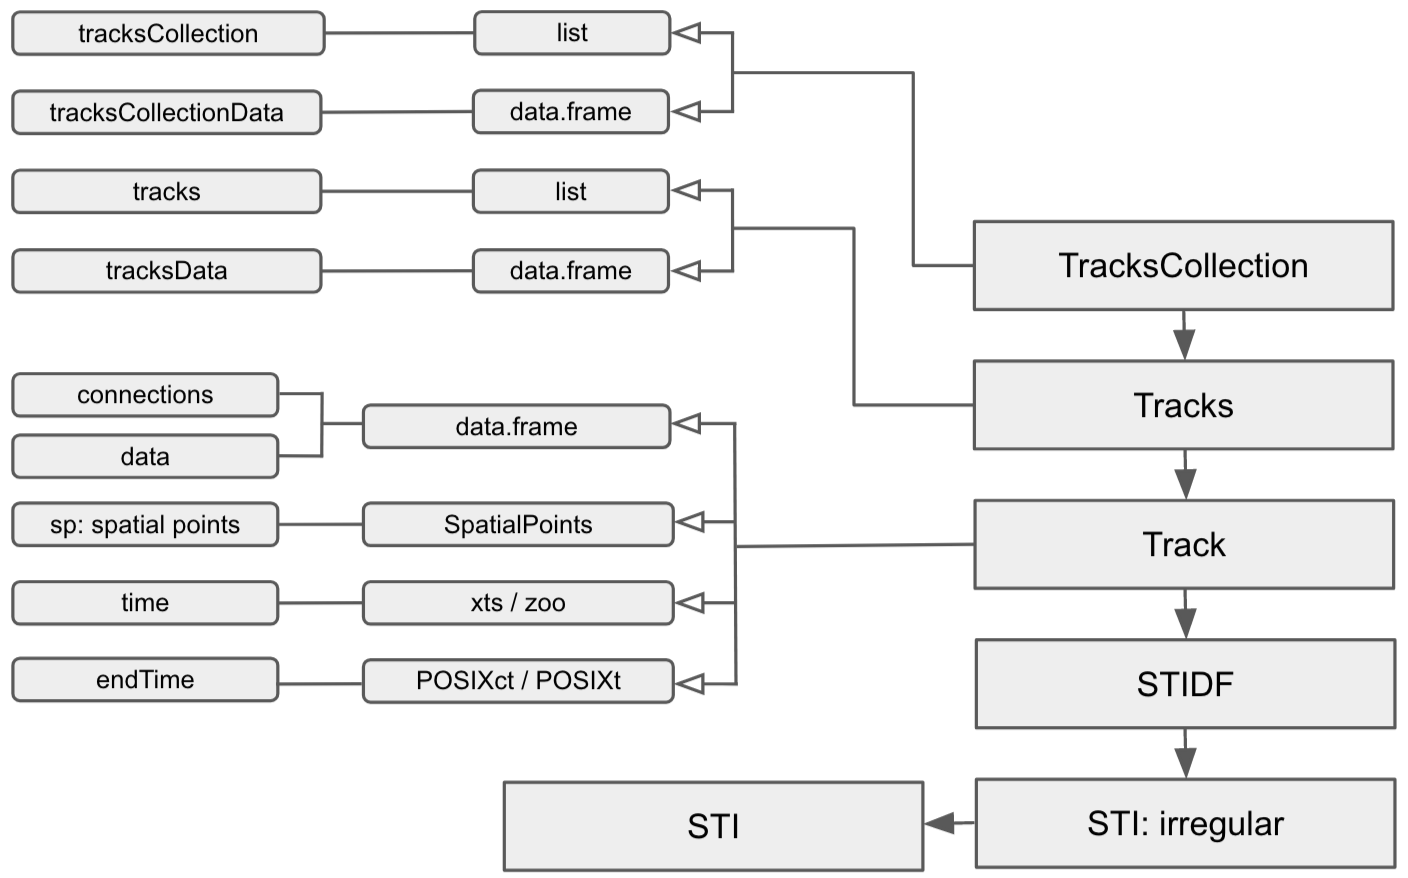
\includegraphics[width = 5in]{classes}
  \caption{Classes for Track data in package \pkg{trajectories}. Solid arrows denote inheritance. Arrows show the corresponding slot's class and slot's names are displayed using lines accordingly.}
  \label{classes}
  \end{figure} 
 
Figure \ref{classes} shows the classes and their connection. We point out that classes \class{STIDF},\class{STI} and \class{ST} belong to the package \pkg{spacetime} inherently .
 % \section{Methods} \label{sec:methods}
 
  A wealth of methods have been implemented to cover the most frequently used use cases. Table \ref{Tablemethod} lists some of the methods applied to the objects of classes \code{Track}, \code{Tracks} and \code{TracksCollection}. Apart from those listed in Table \ref{Tablemethod}, attribute data can be obtained or replaced by using \code{[]}, \code{[[]]}, \code{@} and \code{$}.
  \begin{table}[!h]
  \caption{Methods implemented in \pkg{trajectories} for objects from class \class{Track},\class{Tracks} and \class{TrackCollection}.}
  \begin{center}
  \begin{tabular}{| c | c|}
  \hline
  Method & Operation\\
  \hline
  \code{dim} & Returns the number of spatial points of any track  \\
  \code{summary} & Summarises the internal information\\
  \code{proj4string} & Retrieves projection attributes\\
  \code{coordinates} & Retrieves the coordinates of spatial locations\\
  \code{coordnames}& Retrieves coordinate names of fixes\\
  \code{bbox}& The box (window) which contains the objects\\
  \code{stbox}& The spatio-temporal box (window) which contains the objects\\
   \code{aggregate}& Spatially aggregate track properties (coercing fixes to points)\\
   \code{compare}& Compares two \class{Track} objects: for the common time period\\
 \code{dists}& Compares two \class{Tracks} using the mean distance, the Frechet distance,etc\\
\code{downsample}& Remove fixes from a \class{Track}, starting with the most densely sampled ones\\
\code{frechetDist}& Compute Frechet distance between two \class{Track} objects\\
\code{stcube} & Draw a space-time cube\\
\code{stplot} & Create trellis plot for \class{TracksCollection} objects\\
\code{generalize}& Resample \class{Track} to lower freqency or minimal distance\\
  \hline
  \end{tabular}
  \label{Tablemethod}
  \end{center}
  \end{table}

The use of some methods in Table \ref{Tablemethod} is shown in the following lines of code. Figure \ref{fig:co2consumptionovertime} shows the trellis plot of object \code{Tr} from class \class{TracksCollection} which is previously created. We point out that we have used slot \code{data} of the corresponding tracks as attributes to see their changes over time.
\begin{Schunk}
\begin{Sinput}
R> dim(A1)
\end{Sinput}
\begin{Soutput}
geometries 
         7 
\end{Soutput}
\begin{Sinput}
R> dim(B1)
\end{Sinput}
\begin{Soutput}
geometries 
         6 
\end{Soutput}
\begin{Sinput}
R> stbox(A1)
\end{Sinput}
\begin{Soutput}
    x y                time
min 3 5 2013-09-30 02:00:30
max 7 7 2013-09-30 02:02:31
\end{Soutput}
\begin{Sinput}
R> downsample(A1,B1)
\end{Sinput}
\begin{Soutput}
An object of class Track 
6points 
bbox: 
  min max
x   3   7
y   5   7
Time period: [2013-09-30 02:00:30, 2013-09-30 02:02:31]
\end{Soutput}
\end{Schunk}
\begin{figure}[!h]
\centering
\begin{Schunk}
\begin{Sinput}
R> stplot(Tr, attr = "co2", arrows = TRUE, lwd = 3, by = "IDs")
\end{Sinput}
\end{Schunk}
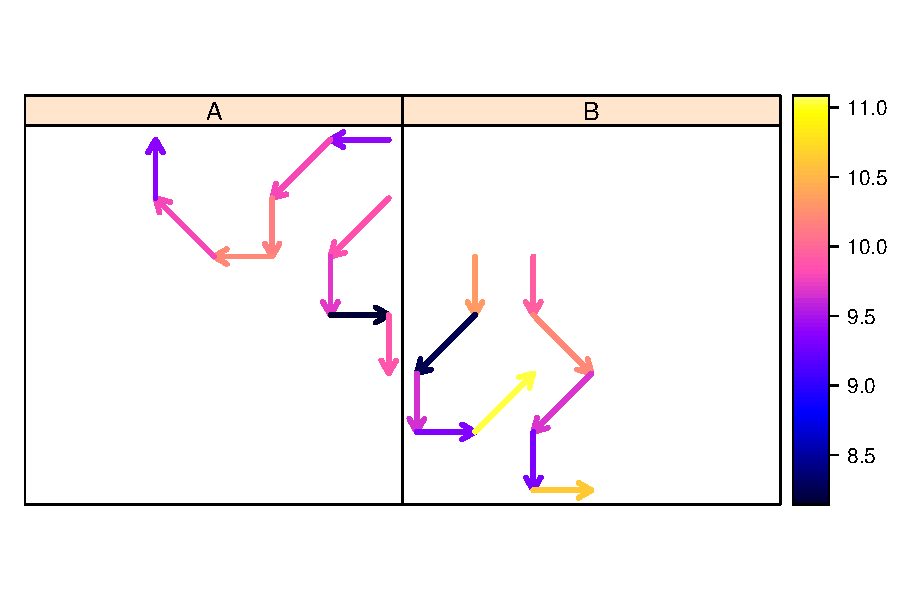
\includegraphics{article-009}
\caption{Co2 consumption over time.}
\label{fig:co2consumptionovertime}
\end{figure}


\section{Simulation and model fitting}\label{simandfitt}
  \subsection{Trajectory simulation}
  Simulating trajectory patterns can be a useful tool to imitate true models and understand their behaviour. The package \pkg{trajectories} allows simulating tracks using \code{rTrack}, \code{rTracks}, \code{rTracksCollection} where \code{rTrack()} generates a single track, \code{rTracks()} simulates a collection of tracks assumed to be passed by a single object and \code{rTracksCollection} is used to simulate a set of tracks passed by different objects. By default, these functions do not consider any box (or window) for the track to be simulated in and consider \code{origin=c(0,0)} as the origin of the track. However, one can still restrict the track to a desirable closed box using the argument \code{bbox}. If \code{transform=TRUE} and no \code{bbox} is given, then \code{rTrack} transforms the track to the default box $[0,1]\times [0,1]$, where in this case the origin is a random point in the default box. If a default box \code{bbox} (e.g. \code{m} in the following example) is given and \code{transform=TRUE}, then \code{origin} is a random point in \code{bbox} and the final track is also transformed into \code{bbox}. The function \code{rTrack} simulates tracks with a predefined number of points per Track (indicated as \code{n} in the code with default $100$). However if \code{nrandom=TRUE} then it simulates a track with a random number of points based on a Poisson distribution with parameter \code{n}. An example of these functions is the following:
\begin{Schunk}
\begin{Sinput}
R> set.seed(10)
R> x <- rTrack();x
\end{Sinput}
\begin{Soutput}
An object of class Track 
100points 
bbox: 
        min       max
x -53.38677 -3.232289
y -53.08787 -1.594295
Time period: [1970-01-01, 1970-01-01 01:39:00]
\end{Soutput}
\begin{Sinput}
R> y <- rTrack(transform = T);y
\end{Sinput}
\begin{Soutput}
An object of class Track 
100points 
bbox: 
  min max
x   0   1
y   0   1
Time period: [1970-01-01, 1970-01-01 01:39:00]
\end{Soutput}
\begin{Sinput}
R> m <- matrix(c(0,10,0,10),nrow=2,byrow = T)
R> w <- rTrack(bbox = m,transform = T);w
\end{Sinput}
\begin{Soutput}
An object of class Track 
100points 
bbox: 
  min max
x   0  10
y   0  10
Time period: [1970-01-01, 1970-01-01 01:39:00]
\end{Soutput}
\begin{Sinput}
R> z <- rTrack(bbox = m,transform = T,nrandom = T);z
\end{Sinput}
\begin{Soutput}
An object of class Track 
108points 
bbox: 
  min max
x   0  10
y   0  10
Time period: [1970-01-01, 1970-01-01 01:47:00]
\end{Soutput}
\end{Schunk}
\begin{figure}[!h]
\begin{center}
\begin{Schunk}
\begin{Sinput}
R> par(mfrow=c(2,2),mar=rep(2.2,4))
R> plot(x,lwd=2,main="x");plot(y,lwd=2,main="y")
R> plot(w,lwd=2,main="w");plot(z,lwd=2,main="z")
\end{Sinput}
\end{Schunk}
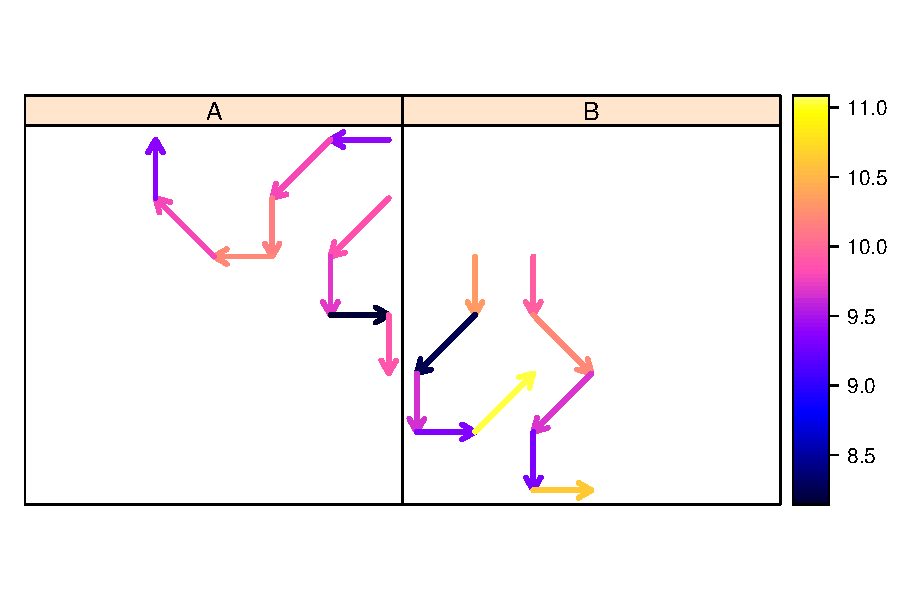
\includegraphics{article-011}
\end{center}
\caption{Simulated random tracks using \code{rTrack}. \code{x} is random track with all defaults. \code{y} is a random track transformed to a unit box. \code{w} is a random track transformed to the box $[0,10]\times [0,10]$ and \code{z} is in a same box as \code{w} but with the random number of points.}
\label{randomtracks}
\end{figure}
Figure \ref{randomtracks} shows four different random tracks: \code{x} is a random track with all defaults, \code{y} is a random track transformed to a unit box, \code{w} is a random track transformed to the box $[0,10]\times [0,10]$, and \code{z} is a simulated track in a same box as \code{w} but with a random number of points. The number of points in \code{w} is $100$ whereas \code{z} is constituted by $108$ points.


 \subsection{Model fitting}
  The behaviour of trajectory data might also be studied using available tools for time series modelling. However, obtaining a proper model is extremely important as it highlights the
  underlying structure of the series, and the fitted model can be used for future forecasting. The \proglang{R} package
  \pkg{trajectories} can fit ARIMA models to movement data. Using \proglang{R} package \pkg{forecast}, the function \code{auto.arima.Track} fits arima models to the spatial coordinates of an object of class \class{Track}. See example below.

\begin{Schunk}
\begin{Sinput}
R> data("Beijing")
R> library(forecast)
R> auto.arima.Track(Beijing[[5]])
\end{Sinput}
\begin{Soutput}
Arima model fitted to x-coordinate: ARIMA(1,0,2) with non-zero mean 
Arima model fitted to y-coordinate: ARIMA(2,1,2) with drift
\end{Soutput}
\end{Schunk}

\section{Exploratory data analysis} \label{sec:explo}
  This section presents some statistical methods, implemented in the \proglang{R} package \pkg{trajectories}, to analyse the behaviour of trajectory patterns. A single plot of trajectories pattern might not display interesting information, and if the pattern contains too many tracks, it then needs some analysis to summarise and reveal concealed information. In particular, one may be interested in discovering the more visited streets within a city. Other interesting findings could be the type of interaction between moving objects over time. In short, having a trajectory pattern, we might be interested in answering the following questions:
  \begin{enumerate}
  \item How does the average distance between objects change over time?
  \item How is the spatially varying distribution of objects?
  \item How do moving objects interact with each other? Does their interaction vary over time?
  \item How does the spatially varying distribution of objects vary over time?
  \end{enumerate}

\subsection{Data}
  We considered a sample of the T-Drive trajectory dataset that contains one-week trajectories of $10357$ taxis during the period of Feb. 2 to Feb. 8, 2008, within Beijing, China. T-drive is a smart driving direction services based on GPS trajectories of a large number of taxis. The GPS-equipped taxis are mobile sensors probing the traffic flows on road surfaces. So, the taxi trajectories contain the information of both human knowledge of experienced drivers and traffic patterns. The total number of points in this dataset is about 15 million and the total distance of the trajectories reaches up to 9 million kilometers. For more details about the data, see \cite{yuan10,yuan11}. 
  
We here point out some useful information about the dataset:
\begin{itemize}
  \item $21$ taxis have no information recorded.
  \item Regardless of taxis with no information, there are $4694$ taxis with less than $10$ recorded locations in at least one day. 
  \item There are tracks with some jumps to the outside of the studied area and it may be caused by lack of GPS accuracy so that wrong locations have been removed. These locations might later be recovered by interpolation.
\end{itemize}
  We thus analyse the cleaned dataset which is based on moving data of $5642$ taxis. The map of the studied area is displayed in Figure \ref{Beijingmapgoogle}.
  \begin{figure}[!h]
  \centering
  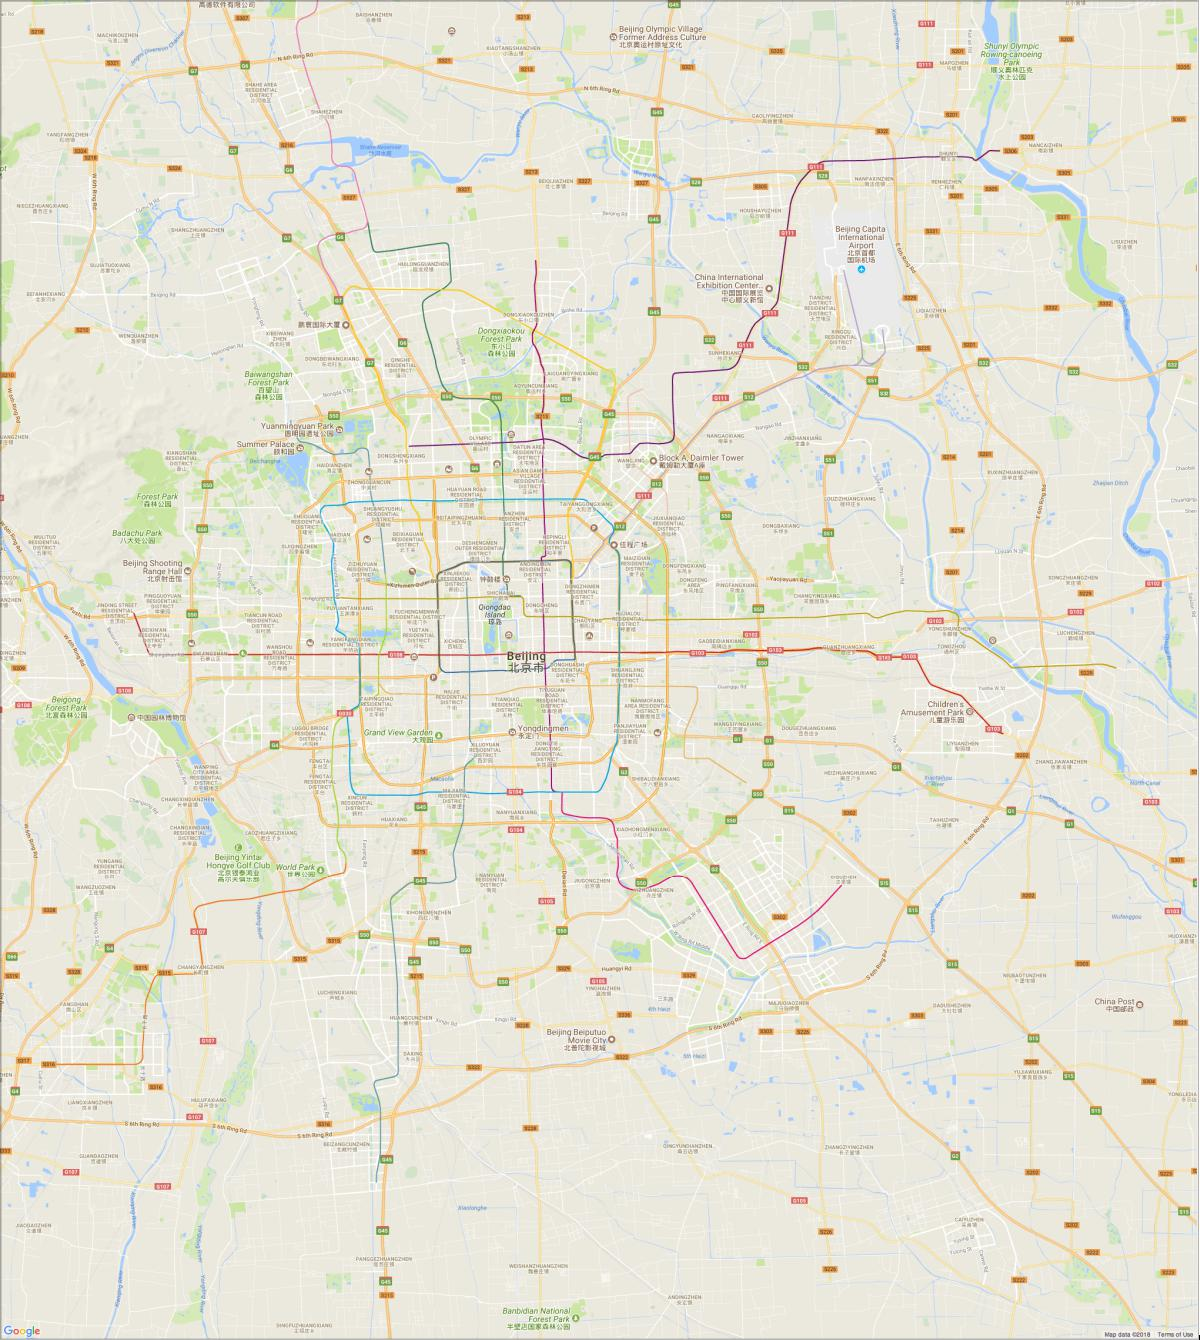
\includegraphics[width = 4in]{Beijingmap}
  \caption{Map of the studied area.}
  \label{Beijingmapgoogle}
  \end{figure}
  
  In the following, we present the implemented methods in \pkg{trajectories} by applying them to the taxi movement dataset in Beijing, China. 
\subsection{Distance analysis}\label{distanal}
  A simple way to get into the nature of movement data is to study the distance between objects. The function \code{dists} provides users with calculating the distance between a pair of objects of class \class{Tracks}. This considers the distance between tracks when they overlap in time. The output is a matrix with distances between each pair of tracks or NA, if they do not overlap in time. A function to calculate distances can be passed to \code{dists}, such as \code{mean}, \code{sum}, \code{frechetDist}, etc.

\begin{Schunk}
\begin{Sinput}
R>  tracks1 <- Tracks(list(Beijing[[1]],Beijing[[2]]))
R>  tracks2 <- Tracks(list(Beijing[[3]],Beijing[[4]]))
R>  dists(tracks1,tracks2,mean)
\end{Sinput}
\begin{Soutput}
         [,1]      [,2]
[1,] 16854.55  9103.338
[2,] 15025.30 10275.476
\end{Soutput}
\end{Schunk}

\subsubsection{Average distance over time}
  The distance between objects over time might discover some interesting information. Studying pairwise distances over time can somehow reveal the type of interaction between objects. Having a pattern of tracks, we may be able to see how moving objects interact each other over time. Moreover, this can highlight the crowded hours within a particular period of time. We here propose to look at average pairwise distances over time. To do so, one can imitate the following steps:
  \begin{leftbar}
  \begin{enumerate}
  \item Based on the time range of all tracks $s_i$, create a regular time sequence.
  \item Interpolate each track $s_i$ based on the created time sequence. For this purpose, the function \code{reTrack} can be used. It reconstructs each track $s_i$ according to a desirable time sequence.
  \item Discretise the trajectory pattern $S$ to a collection of point patterns $\textbf{x}_1,\textbf{x}_2, \ldots, \textbf{x}_k$. Note that the number of points in each pattern might be different.
  \item For any $\mathbf{x}_i ,i=1,\ldots,k$, calculate pairwise distances between all data points.
  \item Report the average of pairwise distances per time.
  \end{enumerate}
  \end{leftbar}
  Steps above are implemented in the function \code{avedistTrack}. In order to use \code{avedistTrack}, we only need to specify the argument \code{timestamp}. It then returns the average distance between objects based on that timestamps. 
\begin{Schunk}
\begin{Sinput}
R> # meandist <- avedistTrack(Beijing,timestamp = "20 mins")
R> # plot(meandist,type="l",lwd=2)
R> # distinframe <- data.frame(tsq=meandist$timeseq,dist=meandist$avedist)
R> # dist3rd <- distinframe[substr(distinframe$tsq,start = 1,stop=10)==
R> #                          "2008-02-03",]
R> # plot(dist3rd$tsq,dist3rd$dist,type="l",xlab="time",
R> #       ylab="average distance",lwd=2)
\end{Sinput}
\end{Schunk}

\begin{figure}[!h]
  \centering
  \subfloat{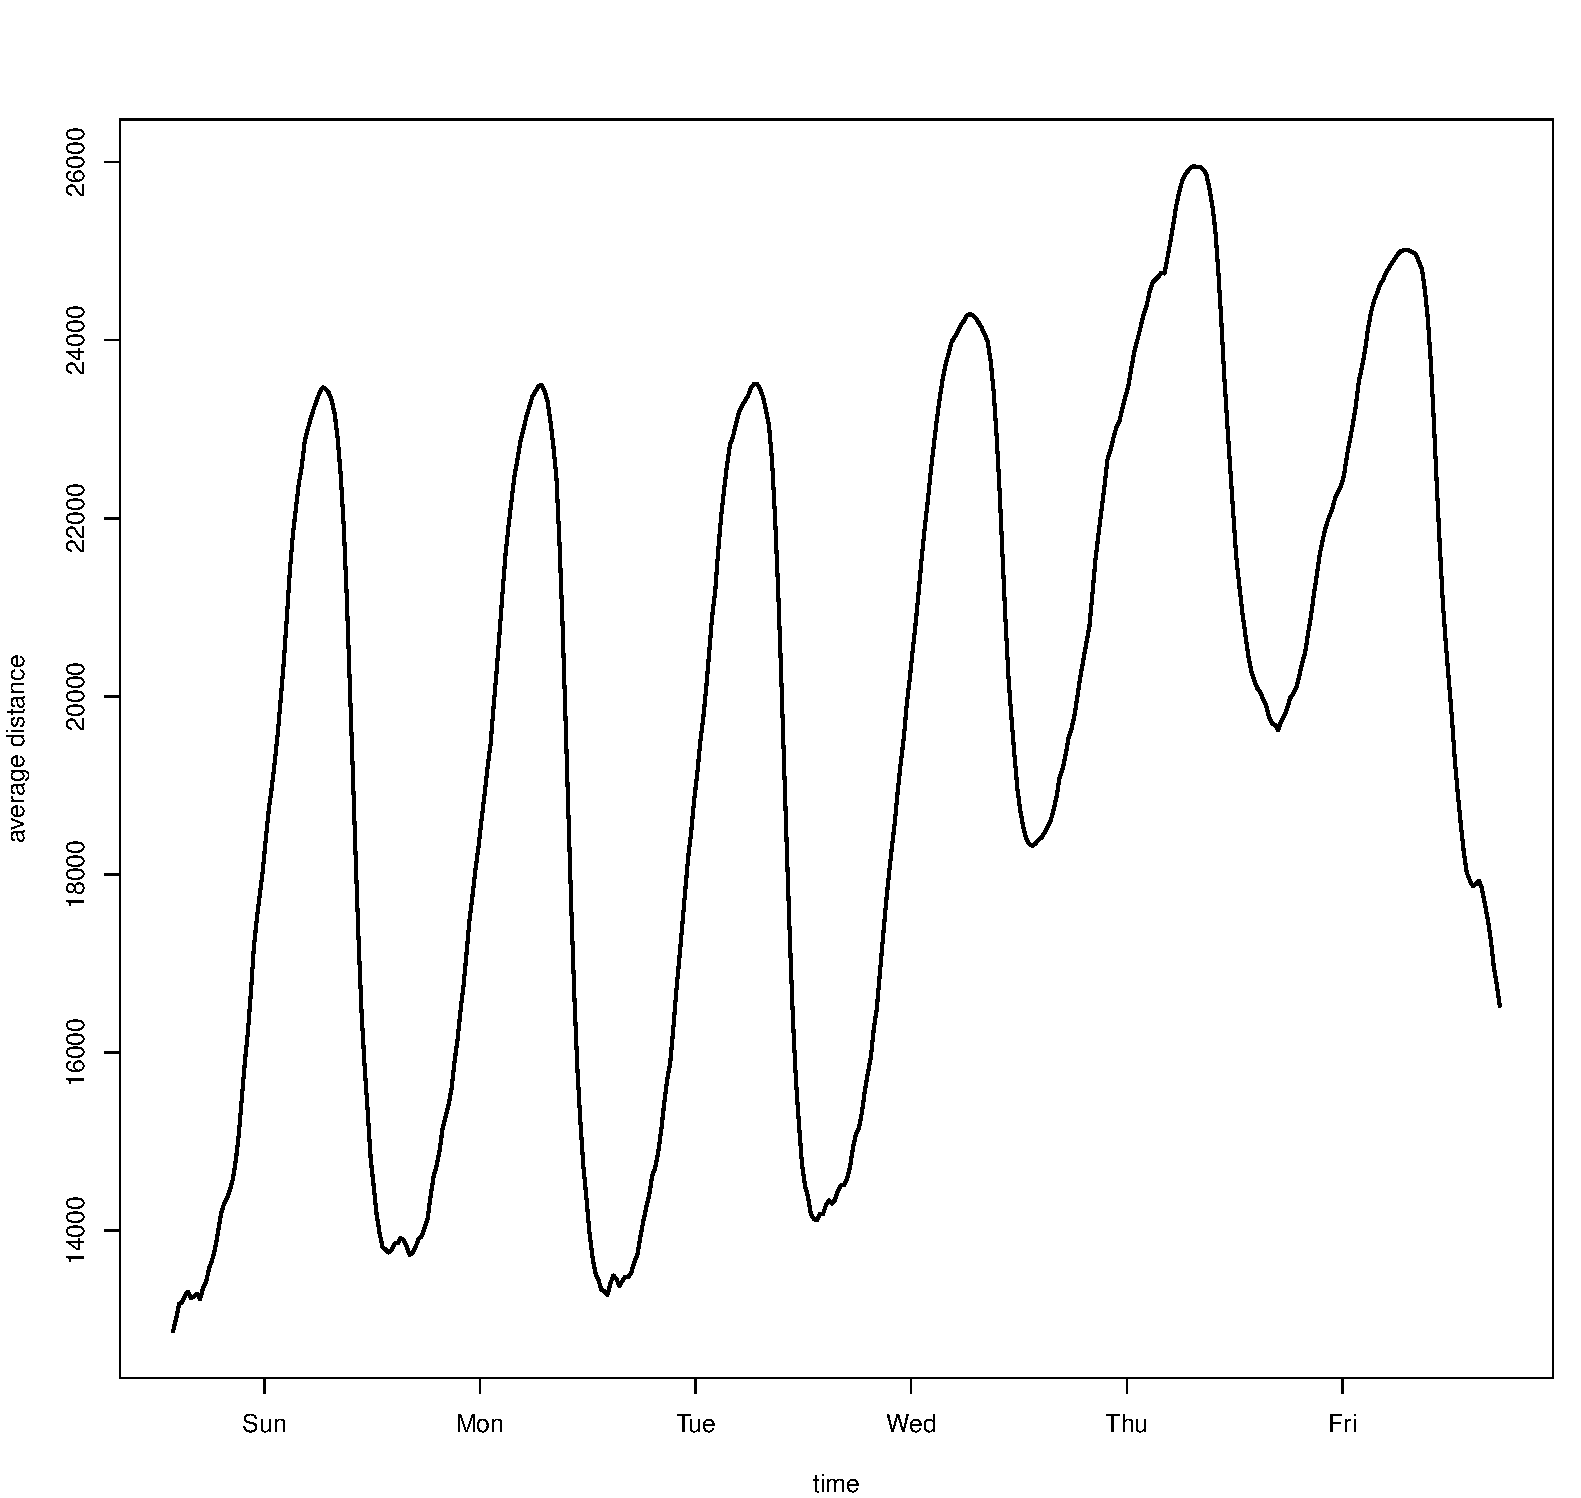
\includegraphics[width = 3.2in]{averagedistance}}
  \subfloat{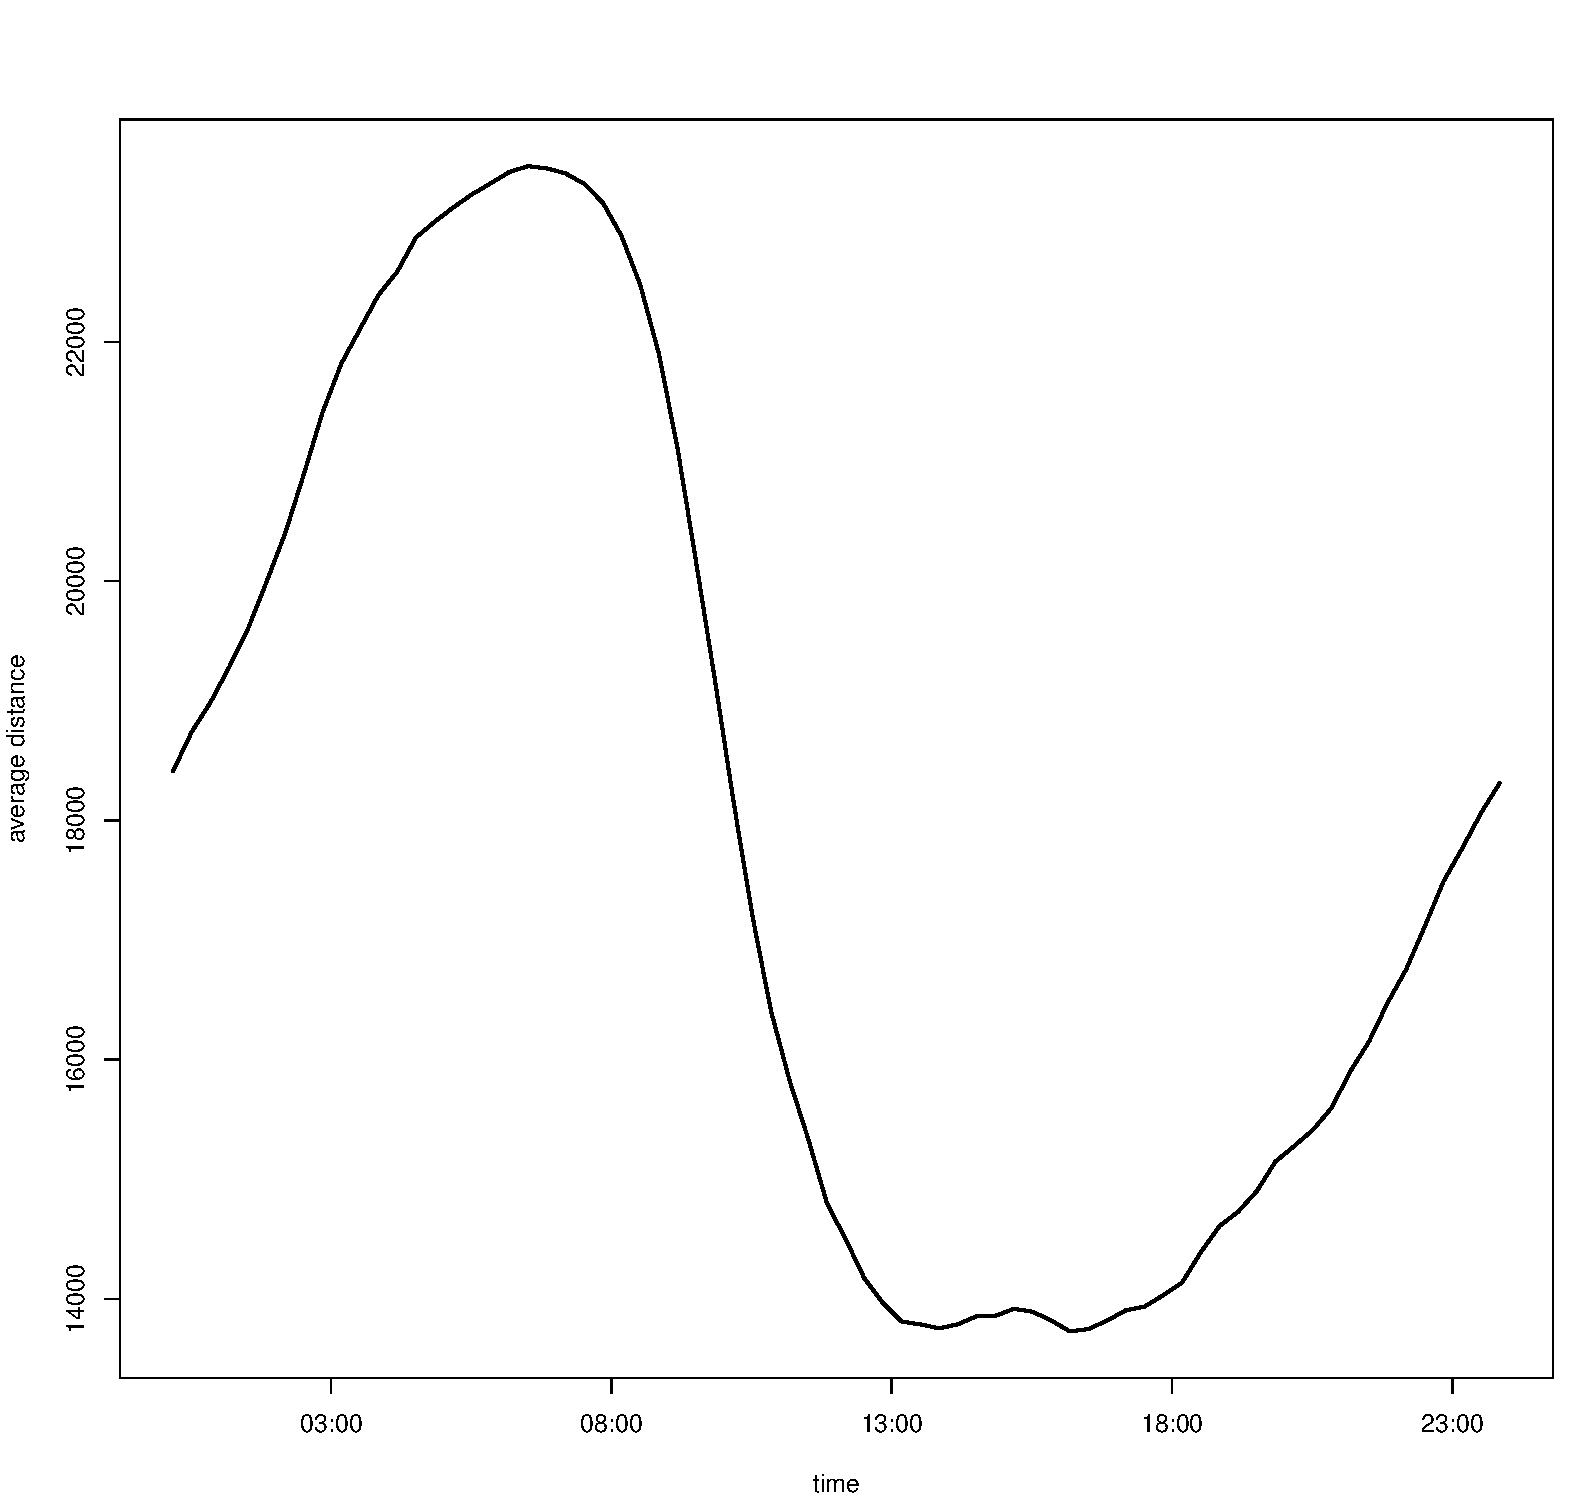
\includegraphics[width = 3.2in]{averagedistance3rd}}
  \caption{Average pairwise distance between taxis in Beijing, China. Left: Within the period 2-8, Feb 2008. Right: During 3rd of Feb 2008.}
  \label{distbijing}
  \end{figure}
Figure \ref{distbijing} shows the average distance between taxis in Beijing. The left plot shows the average pairwise distance between taxis for all the week and it is easily seen that there is a daily trend. In order to see the more crowded hours within a day, we show the average pairwise distances during the 3rd of Feb 2008 in the right plot in Figure \ref{distbijing}. It can be seen that the crowded time comes between midday and 17:00. Also, it shows how taxis are getting far from each other during night. Note that small average distances between taxis might be a sign of traffic during the corresponding hours. We point out that the reason of having larger average distance in the last two days might be the Chinese new year holidays.

As an alternative, one can use nearest neighbour distances instead of pairwise distances. But that might not distinguish patterns with different hot-spots, i.e. patterns with different sets of tracks concentrated in some particular subregions. 
  \subsection{Movement smoothing}
  Aiming at analysing moving objects, it might be of interest to highlight the relationship of movement with  space and time. This section is considered to perform smoothing over the length of movements per each consecutive time. Thus, it might reveal those areas with faster/slower movements. For this purpose, the function \code{Track.idw} performs inverse-distance weighted smoothing over a trajectory pattern by imitating the following steps:
  \begin{leftbar}
  \begin{enumerate}
  \item Follow steps 1-3 in Section \ref{distanal}.
  \item Using each consecutive point patterns, say $\mathbf{x}_o$ and $\mathbf{x}_d$, build $k-1$ segment patterns.
  \item For each segment pattern, find the mid-point of segments, mark it with the length of the corresponding segment.
  \item Using the marked mid-points, create $k-1$ marked point patterns where each mark represents the length of movement per location.
  \item Apply the function \code{idw} from the package \pkg{spatstat} \citep{BRT15} to each marked point pattern where it does inverse-distance weighted smoothing. 
  \item Step 5 returns $k-1$ maps in which the average of them is the output of function \code{Track.idw}.
  \end{enumerate}
  \end{leftbar}
  Mathematically speaking, if for each point pattern $\mathbf{x}_i$, data points $\{ x_1,x_2,\ldots,x_{n_i} \}$ are marked by $\{ l_1,l_2,\ldots,l_{n_i} \}$ then the smoothed value at an arbitrary location $u\in W$ is
  \begin{eqnarray}
  \bar{g}(u)=\frac{1}{k-1} \left[ \sum\limits_{i=1}^{k-1} \frac{\sum\limits_{j=1}^{n_i}w_j l_j}{\sum\limits_{j=1}^{n_i} w_j} \right],
  \end{eqnarray}
  where 
  \begin{eqnarray}
  w_j=\frac{1}{(d(u,x_j))^p},
  \end{eqnarray}
  in which $d$ measures the distance between $u$ and $x_j \in \mathbf{x}_i$, $l_j$ is the corresponding mark of $x_j$ that is the length of the corresponding segment to $x_j$, $n_i$ is the number of points in the $i$th pattern and $p$ is an integer, being 2 as a default value. For details see \cite[Chapter 15]{BRT15}.
  
  In order to use \code{Track.idw}, we only need set the argument \code{timestamp}. When collecting data, it may happen to record the location of objects which are actually stopped. Therefore and to not include them in the movement smoothing, there is an argument \code{epsilon} so that movements with length less than \code{epsilon} are not included in the computation. If no \code{epsilon} is set in the function, it then uses all segments. 
  The following \code{code} generates an image of class \class{im} which reflects the smoothed movement of taxis per 20 minutes.
\begin{Schunk}
\begin{Sinput}
R> # b <- Track.idw(Beijing,timestamp = "20 mins",epsilon=1000)
R> # plot(b,main="",ribwid=0.04,ribsep=0.02)
\end{Sinput}
\end{Schunk}

  \begin{figure}[!h]
  \centering
  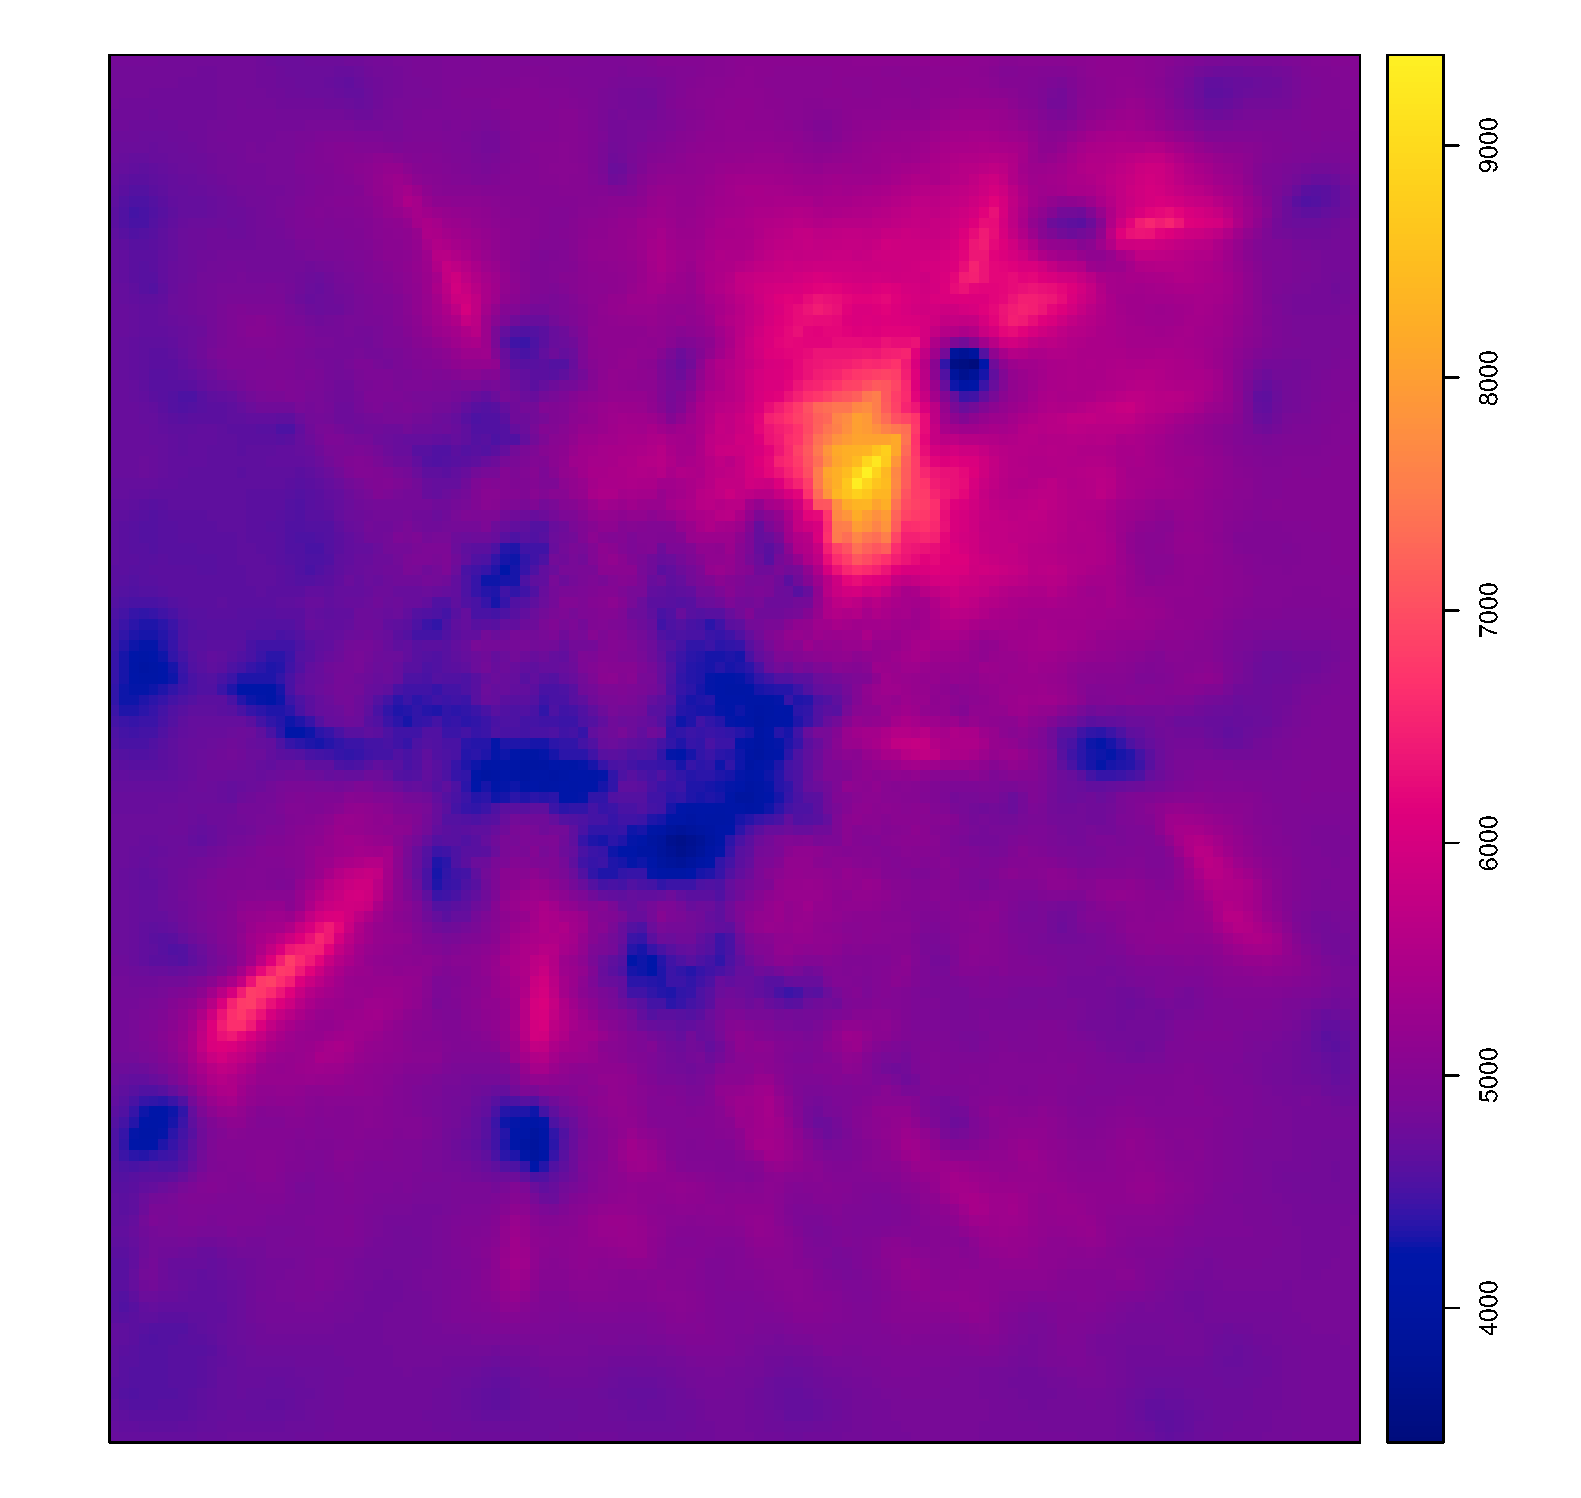
\includegraphics[width = 4in]{idw}
  \caption{Movement smoothing for taxi data in Beijing, China based on \code{timestamp = "20 mins"} and movements with length longer 1000 meters.}
  \label{idwBeijing}
  \end{figure}
  Figure \ref{idwBeijing} shows the movement smoothing for taxi data in Beijing according to the \code{timestamp= "20 mins"}. Here, we have not considered movements with length less than 1000 meters. In other words, we assume taxis with the length of movements less than 1000 meters per 20 minutes as stopped. This confirms that moving in the center is slower than countryside/highways in Beijing, and in particular, it reveals some highways/freeways in which taxis are moving faster.

 After smoothing the length of movements over space, we now turn to see the changes in the average of the length of movements over time. The function \code{avemove} measures the average length of movements passed by a collection of tracks based on a desirable timestamps. Now, we apply this to the taxi data in Beijing as follows
\begin{Schunk}
\begin{Sinput}
R>  # q <- avemove(Beijing,timestamp = "20 mins",epsilon=1000)
R>  # par(mfrow=c(1,2))
R>  # plot(q,type="l",lwd=2)
R>  # qdata <- data.frame(q,attr(q,"tsq")[-c(1,length(attr(q,"tsq")))])
R>  # colnames(qdata) <- c("dist","startingtime")
R>  # q3rd <- qdata[substr(qdata$startingtime,start = 1,stop=10)=="2008-02-03",]
R>  # plot(q3rd$startingtime,q3rd$dist,type="l",xlab="time (hour)"
R>       # ,ylab="average movement",lwd=2)
\end{Sinput}
\end{Schunk}
\begin{figure}[!h]
\centering
\subfloat{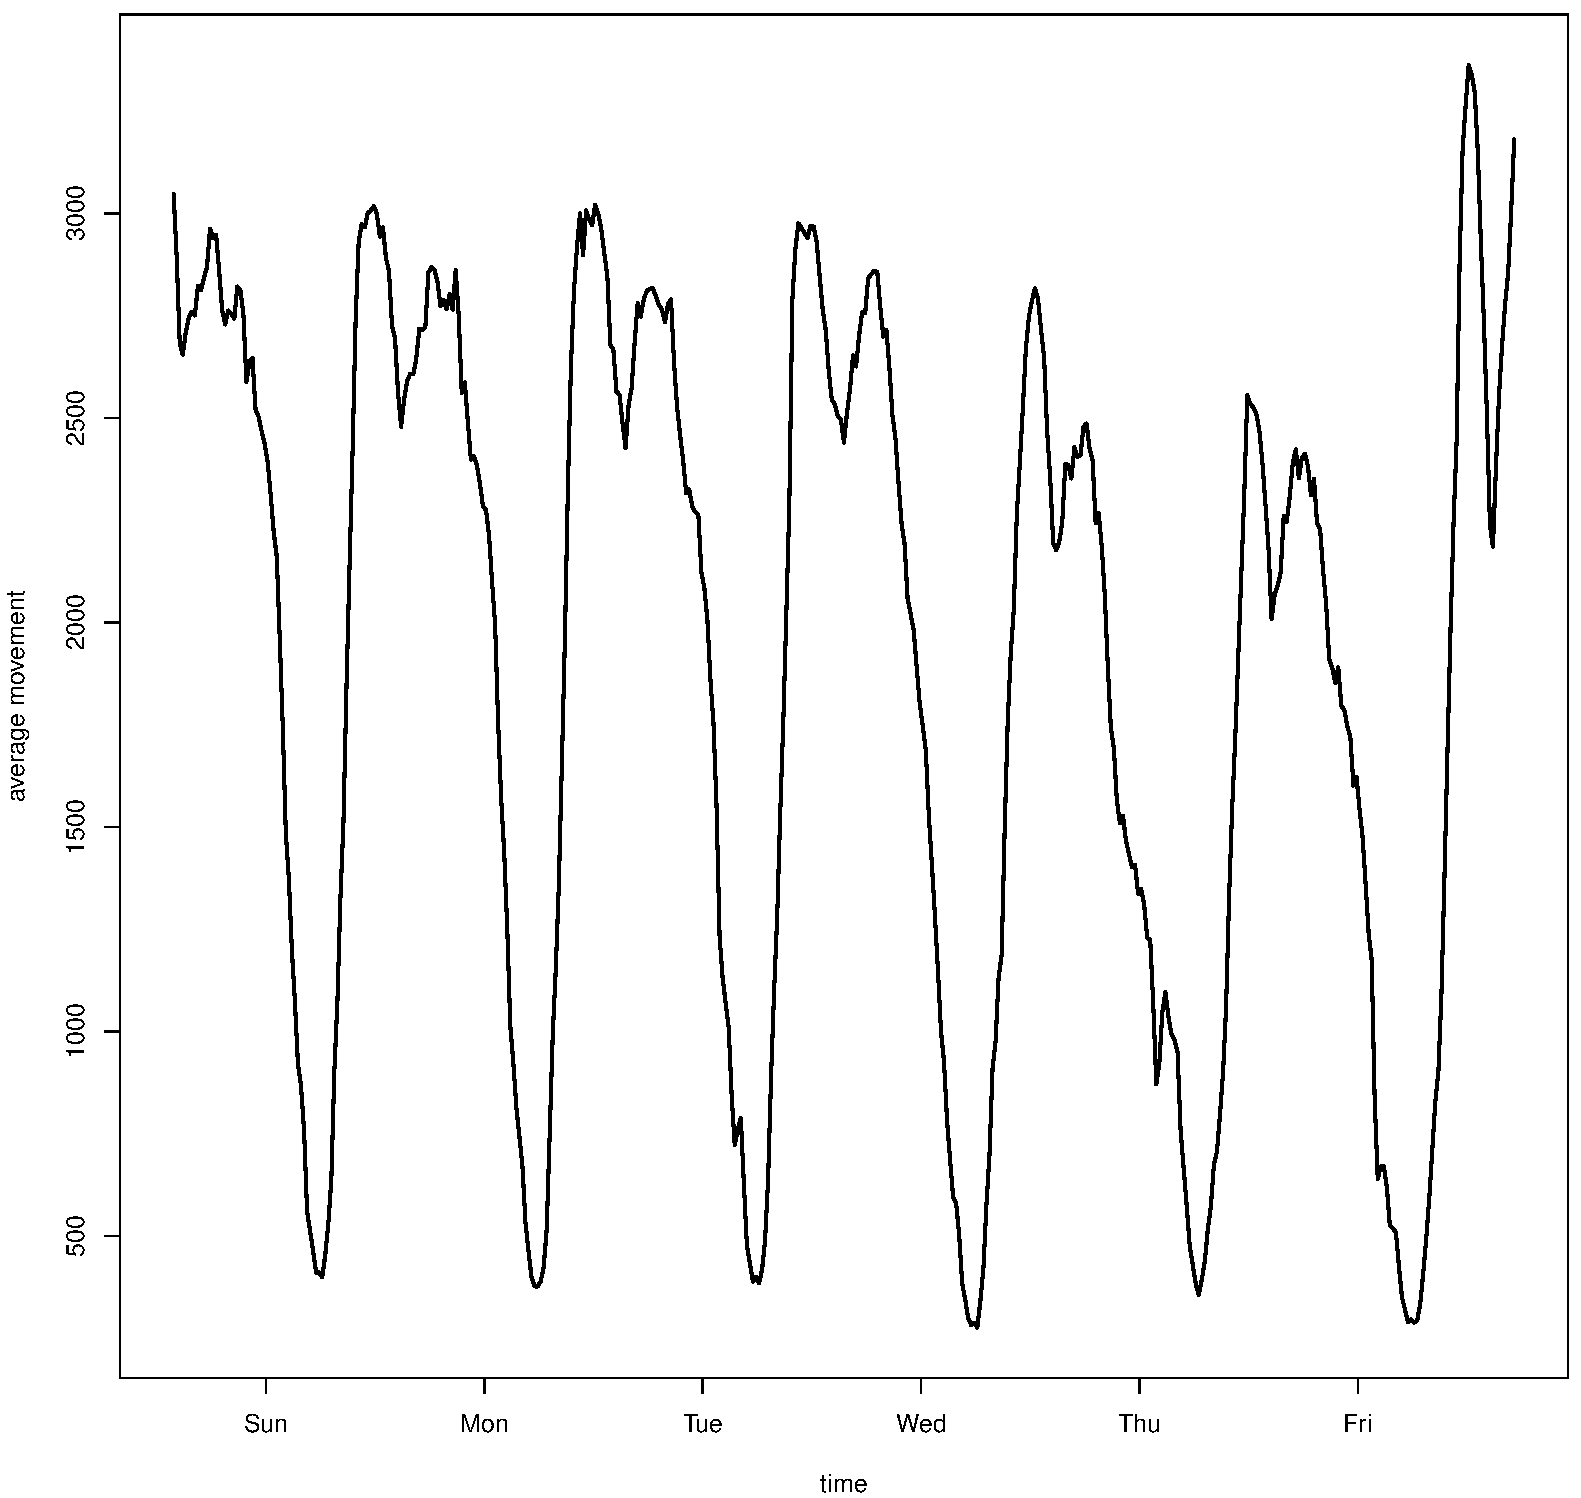
\includegraphics[width = 3.2in]{avemove}}
\subfloat{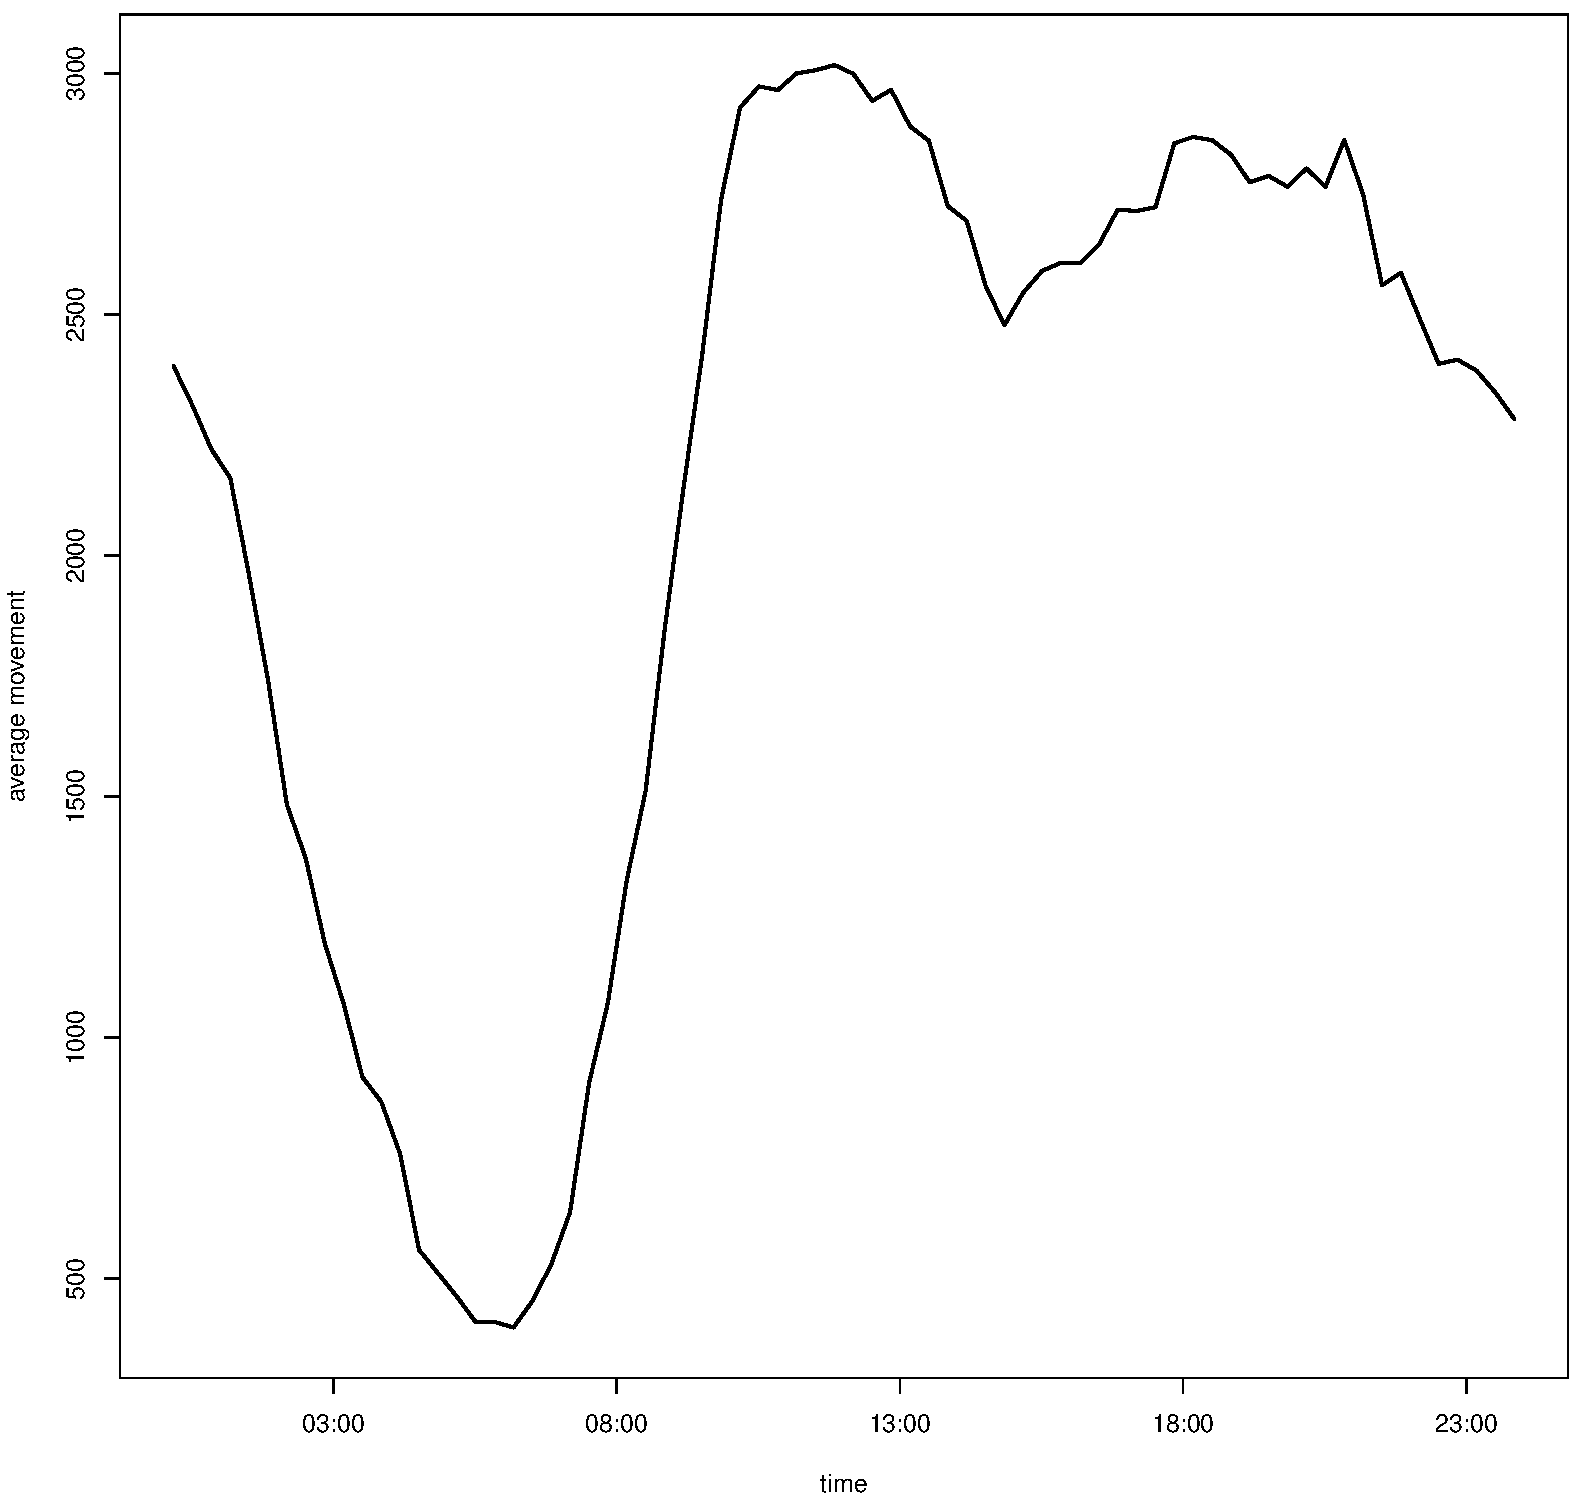
\includegraphics[width = 3.2in]{avemove3rd}}
\caption{Average length of movements by taxis in Beijing, China versus time based on \code{timestamp = "20 mins"}, and movements with length longer than 1000 meters. Left: Within the period 2-8 Feb 2008. Right: During the 3rd of Feb 2008.}
\label{avemovebijing}
\end{figure}
Figure \ref{avemovebijing} shows the average length of movements per 20 minutes by taxis in Beijing. The daily trend can be seen in the left plot, and the right plot shows that between midnight and early morning, the average length of movements is decreasing while from morning till noon there is an increase in the length of movements. In the afternoon, there can be seen a decrease in the average length of movements which might be caused by traffic.

\subsection{Intensity function}\label{sec:intensity}
  An exploratory data analysis of point patterns often starts with estimating the intensity function $\lambda$ which reflects the mean number of points in different regions and may be seen as a ``\textit{heat-map}'' for the events. A well-known method to estimate the intensity function $\lambda$ is by kernel smoothing. \cite{D85} introduced a uniform edge-corrected kernel estimator
  \begin{eqnarray}\label{Uni}
  \widehat{\lambda}(u)=\frac{1}{c_W(u)}\sum\limits_{i=1}^{n} \kappa(u-x_i), \qquad u \in W
  \end{eqnarray}
  and \cite{jones93} proposed the alternative estimator
  \begin{eqnarray}\label{JD}
  \widehat{\lambda}(u)=\sum\limits_{i=1}^{n} \frac{\kappa(u-x_i)}{c_W(x_i)}, \qquad u \in W 
  \end{eqnarray}
  where
  \begin{eqnarray}
  c_W(u)=\int_W \kappa(u-v) \de v, \qquad u \in W
  \end{eqnarray}
  is the edge correction factor, and $\kappa$ is a kernel function. We note that the estimator \eqref{Uni} is unbiased if the true intensity is uniform while the estimator \eqref{JD} conserves mass, meaning that $\int_W \hat{\lambda}(u) \de u =n$. Both estimators \eqref{Uni} and \eqref{JD} can be computed using the \proglang{R} package \pkg{spatstat} for planar point patterns. We here avoid mathematical definitions of a point process and assume that $X$ is finite, i.e. any realisation is a point pattern with finite number of points, and the number of points in any subregion is a well-defined random variable \citep{BRT15}. For technical details of point processes see \citep{MW03,daley07}.
  
  Being able to estimate the intensity function of planar spatial point patterns, we are here interested in estimating the intensity function for trajectory patterns. Such estimator can highlight well-traveled areas based on the tracks of moving objects (e.g.\ humans, cars). We next propose an average intensity estimate using the following steps:
  \begin{leftbar}
  \begin{enumerate}
  \item Follow steps 1-3 as in Section \ref{distanal}.
  \item For any $\textbf{x}_i$, estimate the intensity function, say, $\lambda_i$.
  \item The average over all estimated intensity functions $\widehat{\lambda}_i$ may be considered as an estimated intensity for the trajectory pattern $S$.
  \end{enumerate}
  \end{leftbar}
  Mathematically speaking, and (for instance) using the intensity estimator \eqref{JD}, we propose
  \begin{eqnarray}\label{Trackest}
  \widehat{\widehat{\lambda}}(u)=\frac{1}{k} \sum\limits_{i=1}^{k} \widehat{\lambda}_i(u) =\frac{1}{k}\sum\limits_{i=1}^{k} \sum\limits_{j=1}^{n_i} \frac{\kappa(u-x_j)}{c_W(x_j)}, \qquad u \in W,
  \end{eqnarray}
  as an estimator of the intensity of the trajectory pattern $S$. Intuitively, we interpret $\widehat{\widehat{\lambda}}(u)$ as the average expected number of points (objects) within the time period $T$ in a small area around $u$. As a simple example, consider the movements of cars within a city in a particular day, the estimator \eqref{Trackest} reveals the more dense streets, highways, freeways, etc in that day. Intensity estimators \eqref{Uni} and \eqref{JD} are implemented in the \pkg{trajectories} package using the function \code{density.Track}. The function \code{density.Track} builds the point patterns $\textbf{x}_1,\textbf{x}_2, \ldots, \textbf{x}_k$ and pass them to the function \code{density.ppp} in the package \pkg{spatstat}.

We next turn to calculate the average estimated intensity of the taxi data using the estimator \eqref{Trackest}.

\begin{Schunk}
\begin{Sinput}
R> # d <- density.Track(Beijing,timestamp = "20 mins",bw.ppl)
R> # par(mfrow=c(1,2))
R> # plot(d,main="",ribwid=0.04,ribsep=0.02)
R> # #focus on the center
R> # w <- owin(c(440000,455000),c(4410000,4430000))
R> # pps <- attr(d,"ppps")
R> # npps <- lapply(X=1:length(pps),FUN = function(i){
R> #   pps[[i]][w]
R> # })
R> # 
R> # centerimg <- lapply(X=1:length(npps),FUN = function(i){
R> #   density(npps[[i]],bw.ppl(npps[[i]]))
R> # })
R> # fcenterimg <- Reduce("+",centerimg)/length(centerimg)
R> # 
R> # plot(fcenterimg,main="",ribwid=0.04,ribsep=0.02)
\end{Sinput}
\end{Schunk}
Figure \ref{bijingint} shows the estimated intensity using the estimator \eqref{Uni} for both Beijing and its metropolitan area. The bandwidth has been selected using a likelihood cross-validation method and the function \code{bw.ppl} in \pkg{spatstat}. Other bandwidth selection methods can also be passed to \code{density.Track}. Figure \ref{bijingint} highlights the most well-traveled areas in which those areas in the countryside with higher intensities (left plot) are some townships or airports. The right plot highlights the crowded routes within the center of Beijing.
  \begin{figure}[!h]
  \centering
  \subfloat{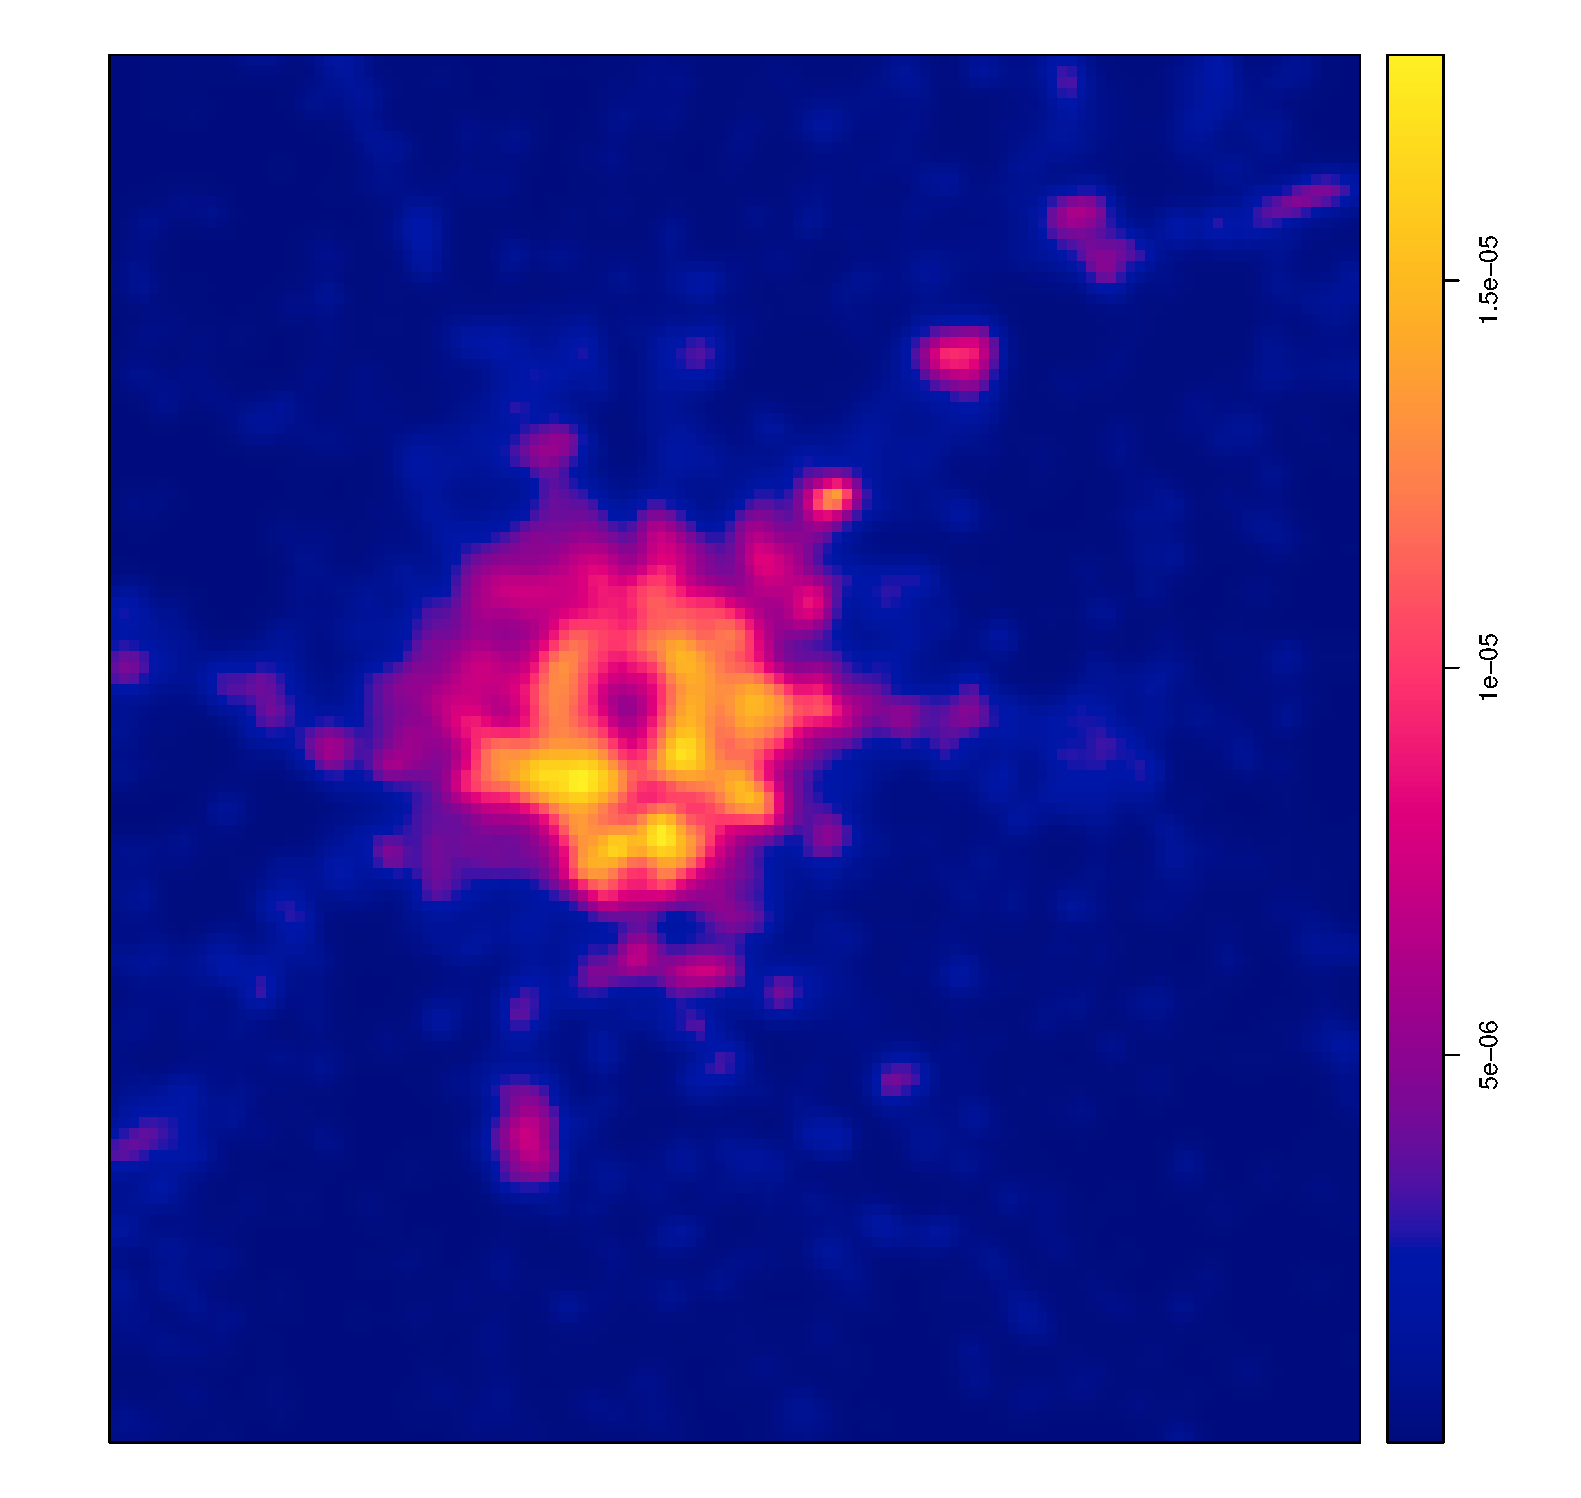
\includegraphics[width = 3.3in]{Intensity}}
  \subfloat{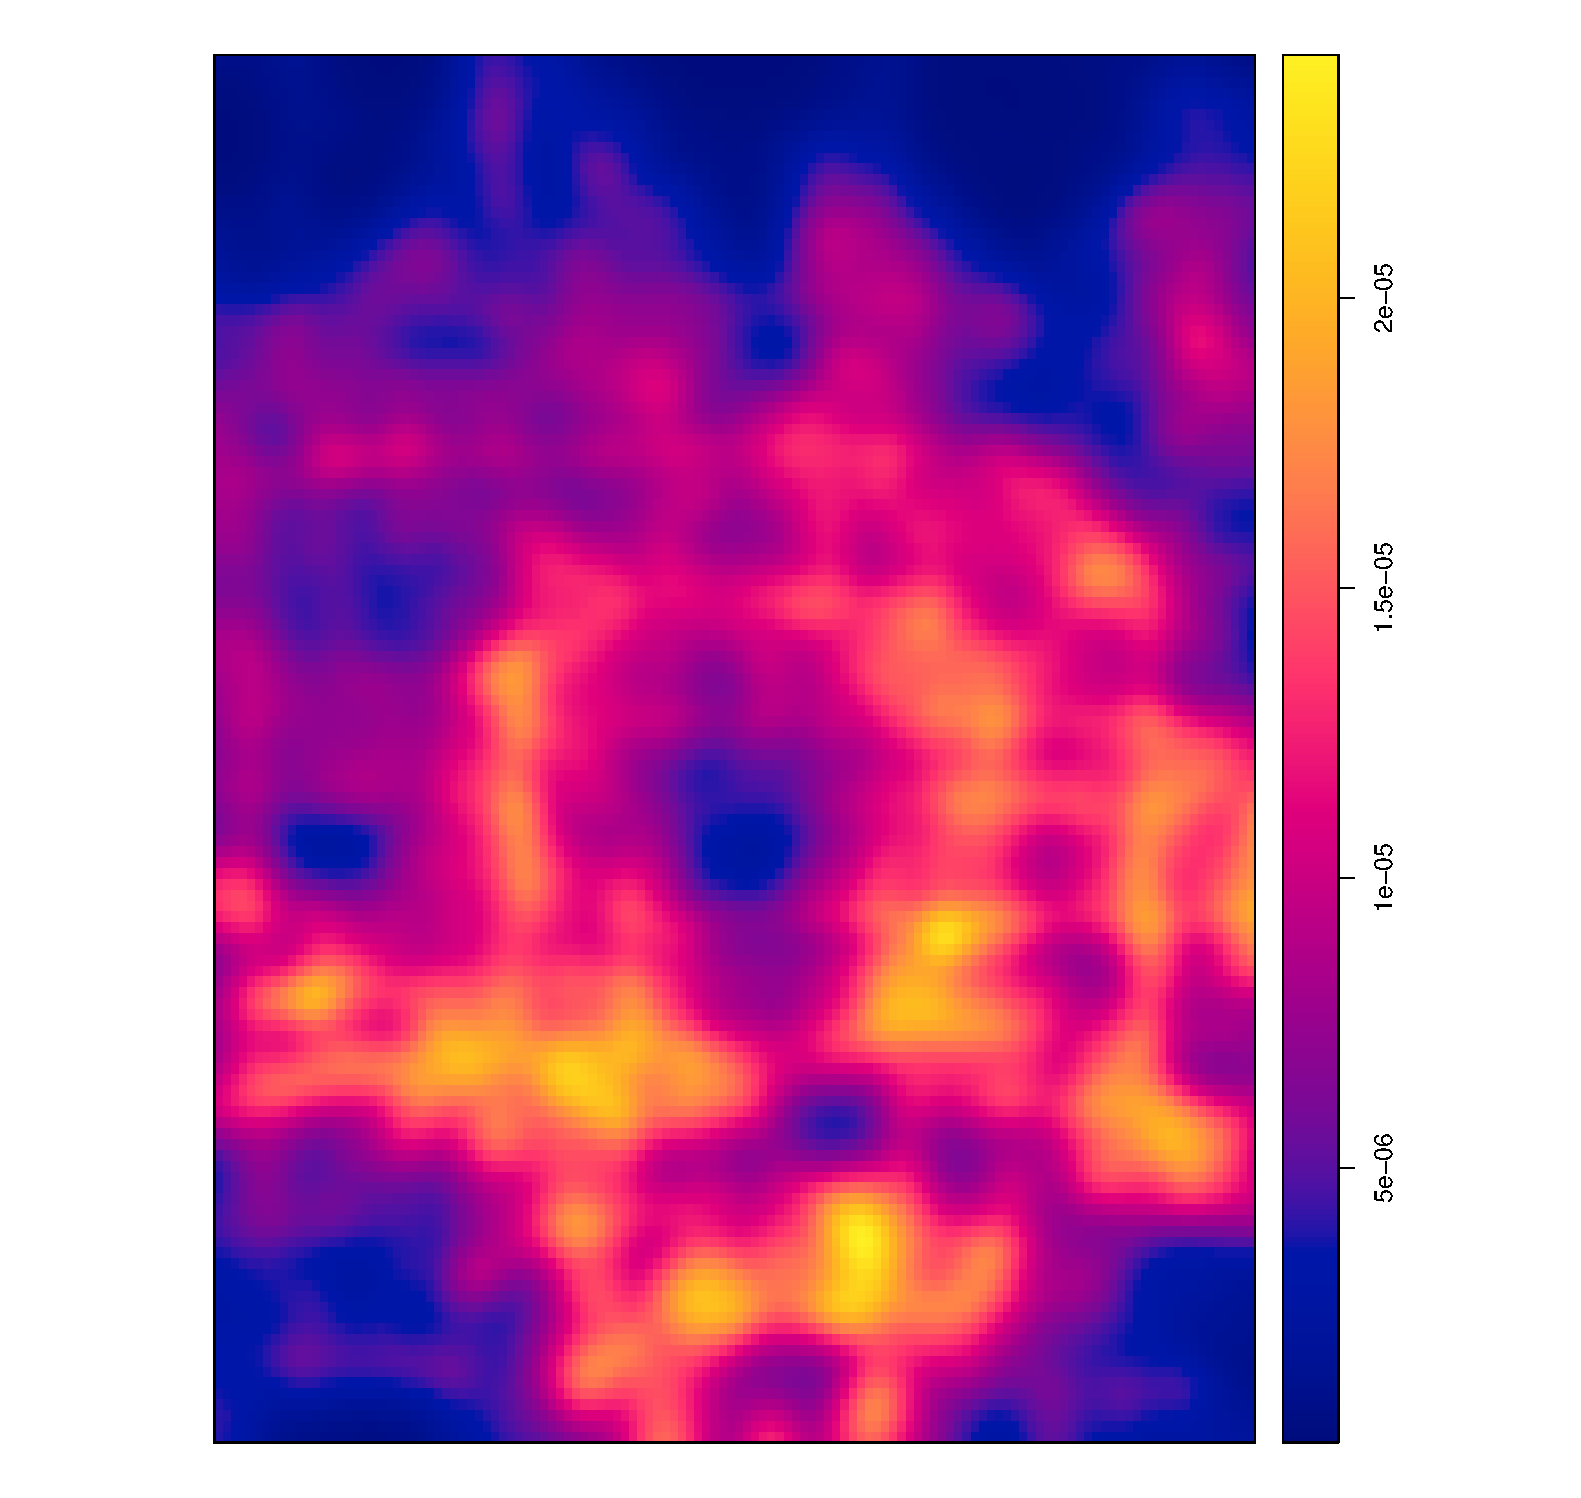
\includegraphics[width = 3.3in]{Intensitycenter}}
  \caption{Estimated intensity function. Left: Beijing. Right: Beijing metropolitan area.}
  \label{bijingint}
  \end{figure}

One may still think of adaptive intensity estimators such as the Voronoi estimator \citep{Ord78,BSV10}. We here point out that as the estimator \eqref{Trackest} is built based on an average of estimated intensity functions of a set of spatial point patterns, one can estimate each of $\lambda_i$ using adaptive estimators resulting in a final adaptive estimator for the corresponding trajectory pattern.
  \subsection{Chi maps}
  After discretising the trajectory pattern $S$ to some point patterns and being able to estimate the individual intensity functions $\lambda_i$, one may think of discovering the areas with more/less events than the expected number. This motivates us to think of $\chi^2$ statistics 
  \begin{eqnarray}\label{chistat}
  \chi^2 =\frac{o-e}{\sqrt[]{e}},
  \end{eqnarray}
  which measures the discrepancy between the expected number $(e)$ and observed number $(o)$. This can be easily applied to the estimated intensity functions $\widehat{\lambda}_1,\widehat{\lambda}_2,\ldots,\widehat{\lambda}_k$ and in any time $t_i, i=1,\ldots,k$, and as a result we can see where the estimated intensity differs from the expected intensity. For example, for a fixed time $t=t_1$,
  \begin{eqnarray*}
  e_{t_1}(u)=\frac{\sum\limits_{i=1}^k \widehat{\lambda}_i(u) \sum\limits_{v \in W} \widehat{\lambda}_1(v)}{\sum\limits_{i=1}^{k}\sum\limits_{v \in W} \widehat{\lambda}_i (v)}, \qquad u \in W,
  \end{eqnarray*}
  is the expected intensity at time $t=t_1$ and location $u \in W$. Doing so for all $u \in W$ enables us to draw a map of $\chi^2$ values in a fixed time. The resulting map discloses the areas where the estimated intensity differs from the expected intensity. The function \code{chimaps} generates a map based on a given timestamp and rank. The argument rank is a number between one and the length of the generated time sequence based on the given timestamp.
  
  The chi maps of the 3rd of Feb based on three different ranks are displayed in Figure \ref{bijingchi}. Values of each pixel is calculated by equation \eqref{chistat}.  We show the chi maps for three different times during the day in which changes over time can be seen. The left plot of Figure \ref{bijingchi} shows the chi map at \code{06:10:44} so that the estimated intensity is higher than the expected intensity in the countryside. The reason for this might be the movements from countryside to the city center in the early morning. The middle plot of Figure \ref{bijingchi} shows that the estimated intensity in the city is higher than the expected intensity. This may be caused  by heavier traffic in the city during the day than in the countryside. In the right plot of Figure \ref{bijingchi}, although the estimated intensity is still slightly higher than the expected one in the city, can see that the $\chi^2$ statistic \eqref{chistat} takes values around 0 almost everywhere at night. These three plots together confirm the changes in the values of the $\chi^2$ statistic \eqref{chistat} over time so that the mass is moving to the city in the morning and goes away in the evening. This behaviour may be explained by the movements to the city in the the morning and moving back to the countryside in the evening.

\begin{Schunk}
\begin{Sinput}
R> # ch <- chimaps(Beijing,timestamp = "20 mins",rank = 200)
R> # chall <- attr(ch,"ims")
R> # minmax <- mclapply(X=1:length(chall),function(i){
R> #     return(list(min(chall[[i]]$v),max(chall[[i]]$v)))
R> #   })
R> # minmax <- do.call("rbind",minmax)
R> # col5 <- colorRampPalette(c('blue','white','red'))
R> # color_levels=200 
R> # par(mar=c(0,0,1,1))
R> # plot(chall[[51]],zlim=c(-max(abs(unlist(minmax))),max(abs(unlist(minmax))))
R> #           ,main=attr(ch,"timevec")[51],ribwid=0.04,ribsep=0.02,
R> #           col=col5(n=color_levels))
R> # plot(chall[[75]],zlim=c(-max(abs(unlist(minmax))),max(abs(unlist(minmax))))
R> #           ,main=attr(ch,"timevec")[75],ribwid=0.04,ribsep=0.02,
R> #           col=col5(n=color_levels))
R> # plot(chall[[104]],zlim=c(-max(abs(unlist(minmax))),max(abs(unlist(minmax))))
R> #           ,main=attr(ch,"timevec")[104],ribwid=0.04,ribsep=0.02,
R> #           col=col5(n=color_levels))
\end{Sinput}
\end{Schunk}

\begin{figure}[!h]
  \centering
  \subfloat{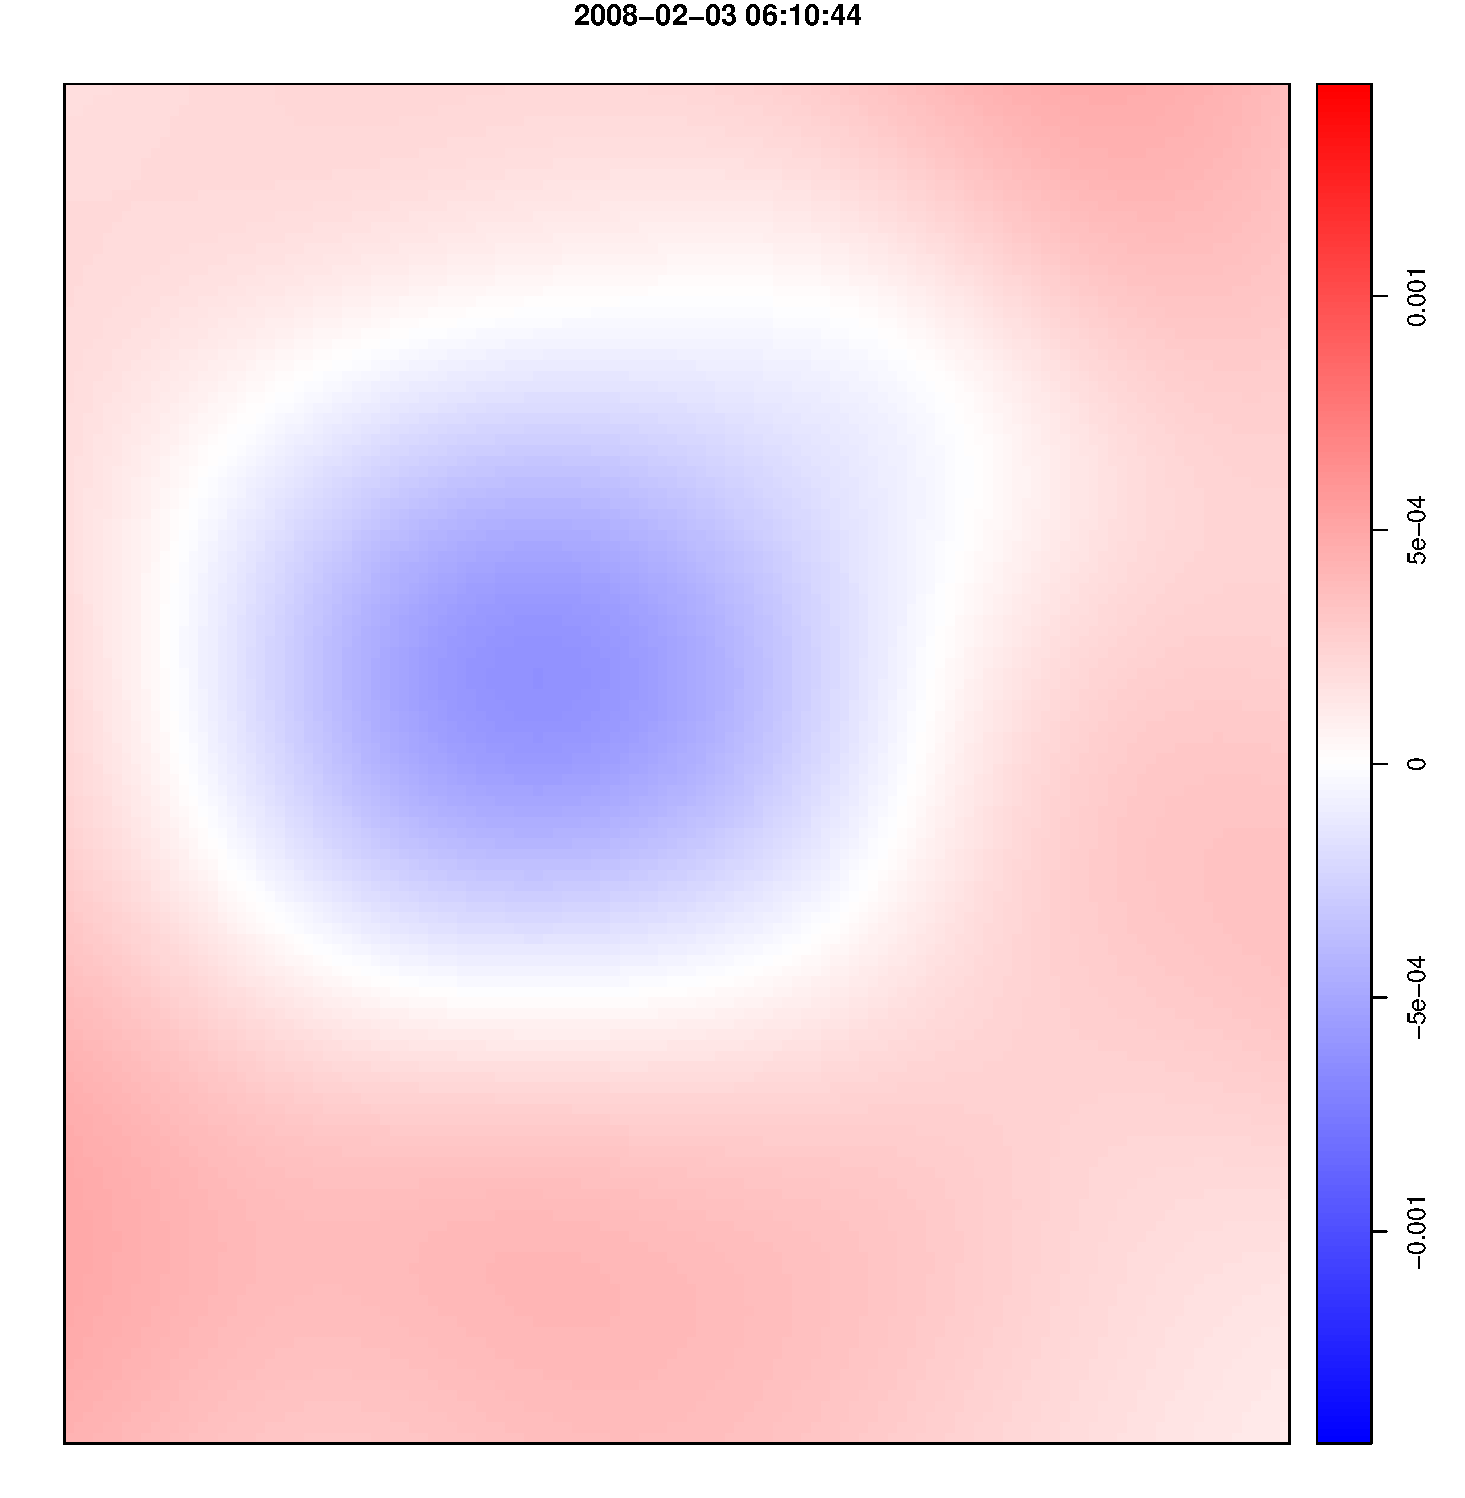
\includegraphics[width = 2.2in]{chi1}}
  \subfloat{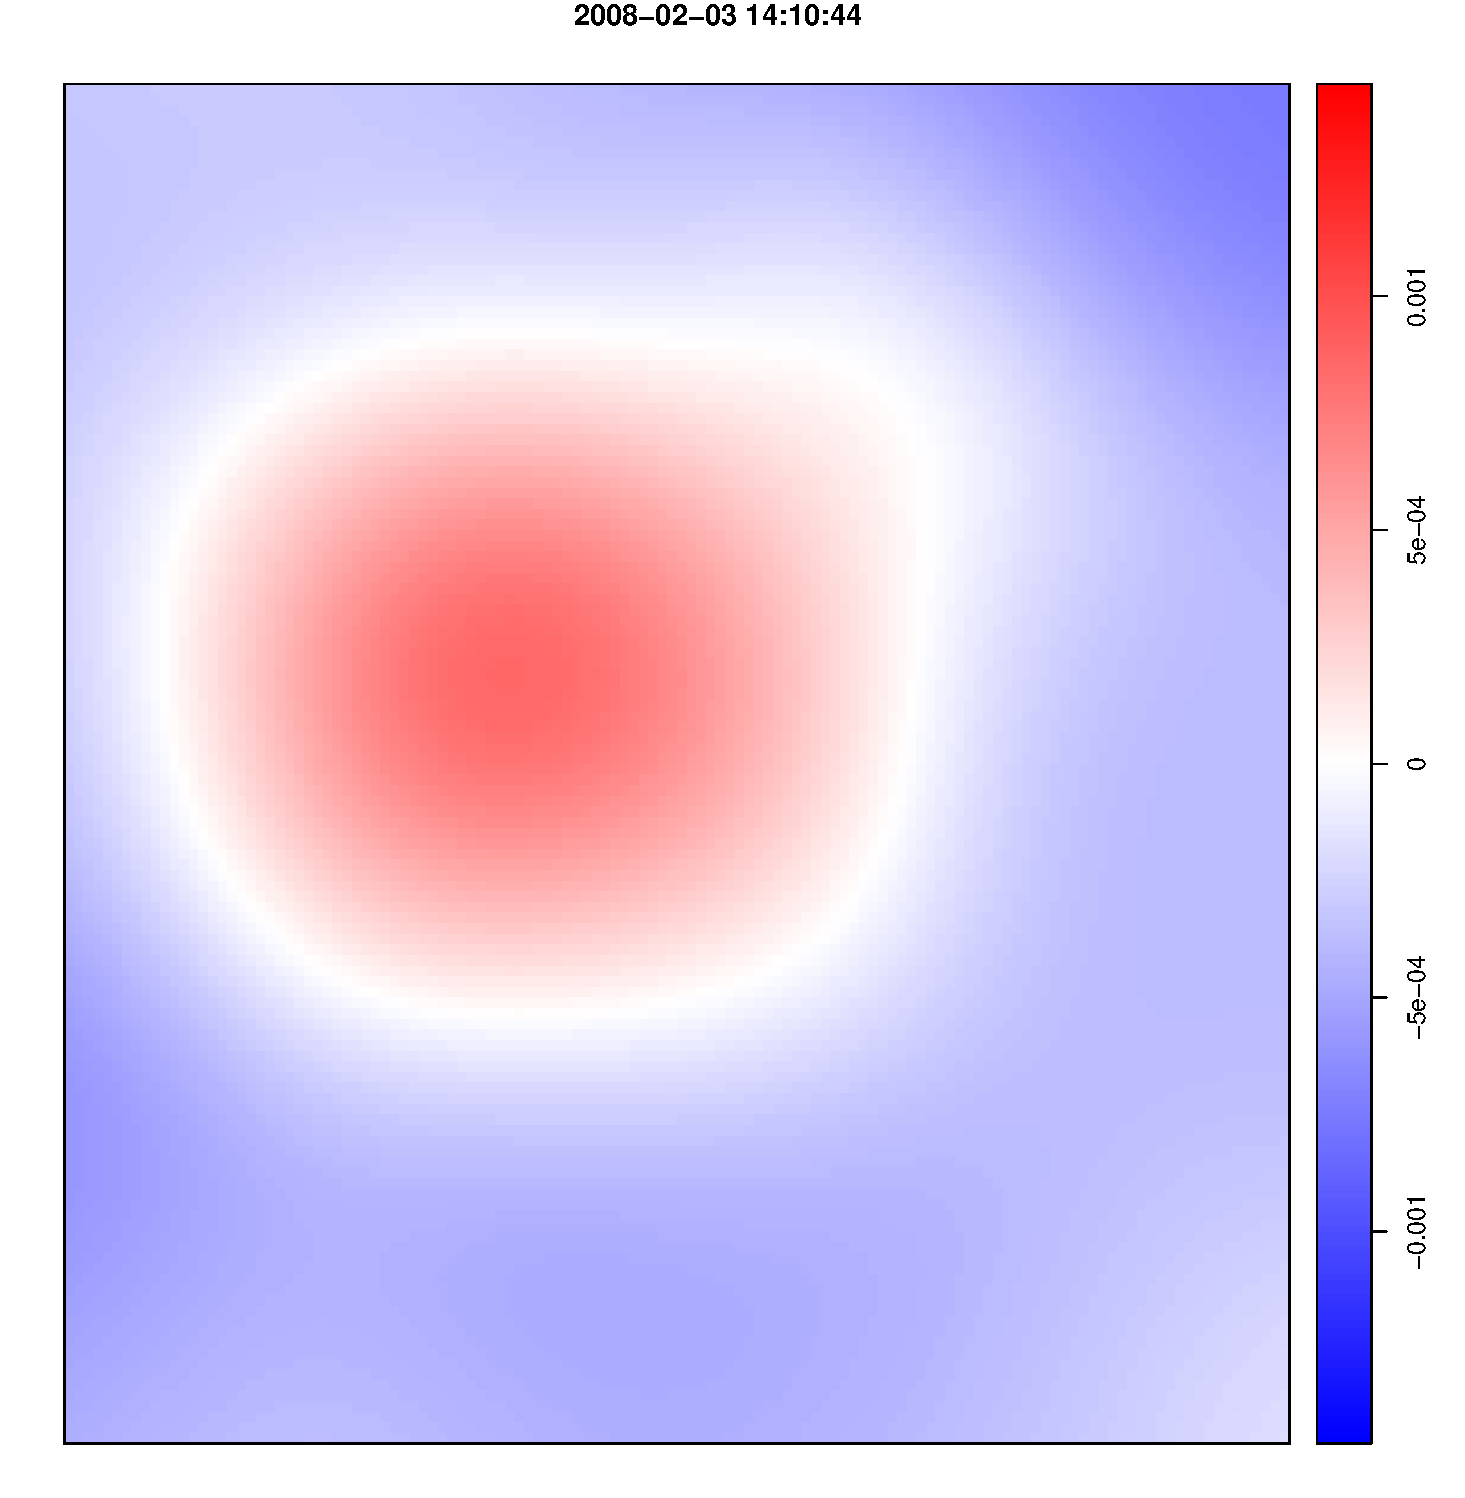
\includegraphics[width = 2.2in]{chi2}}
  \subfloat{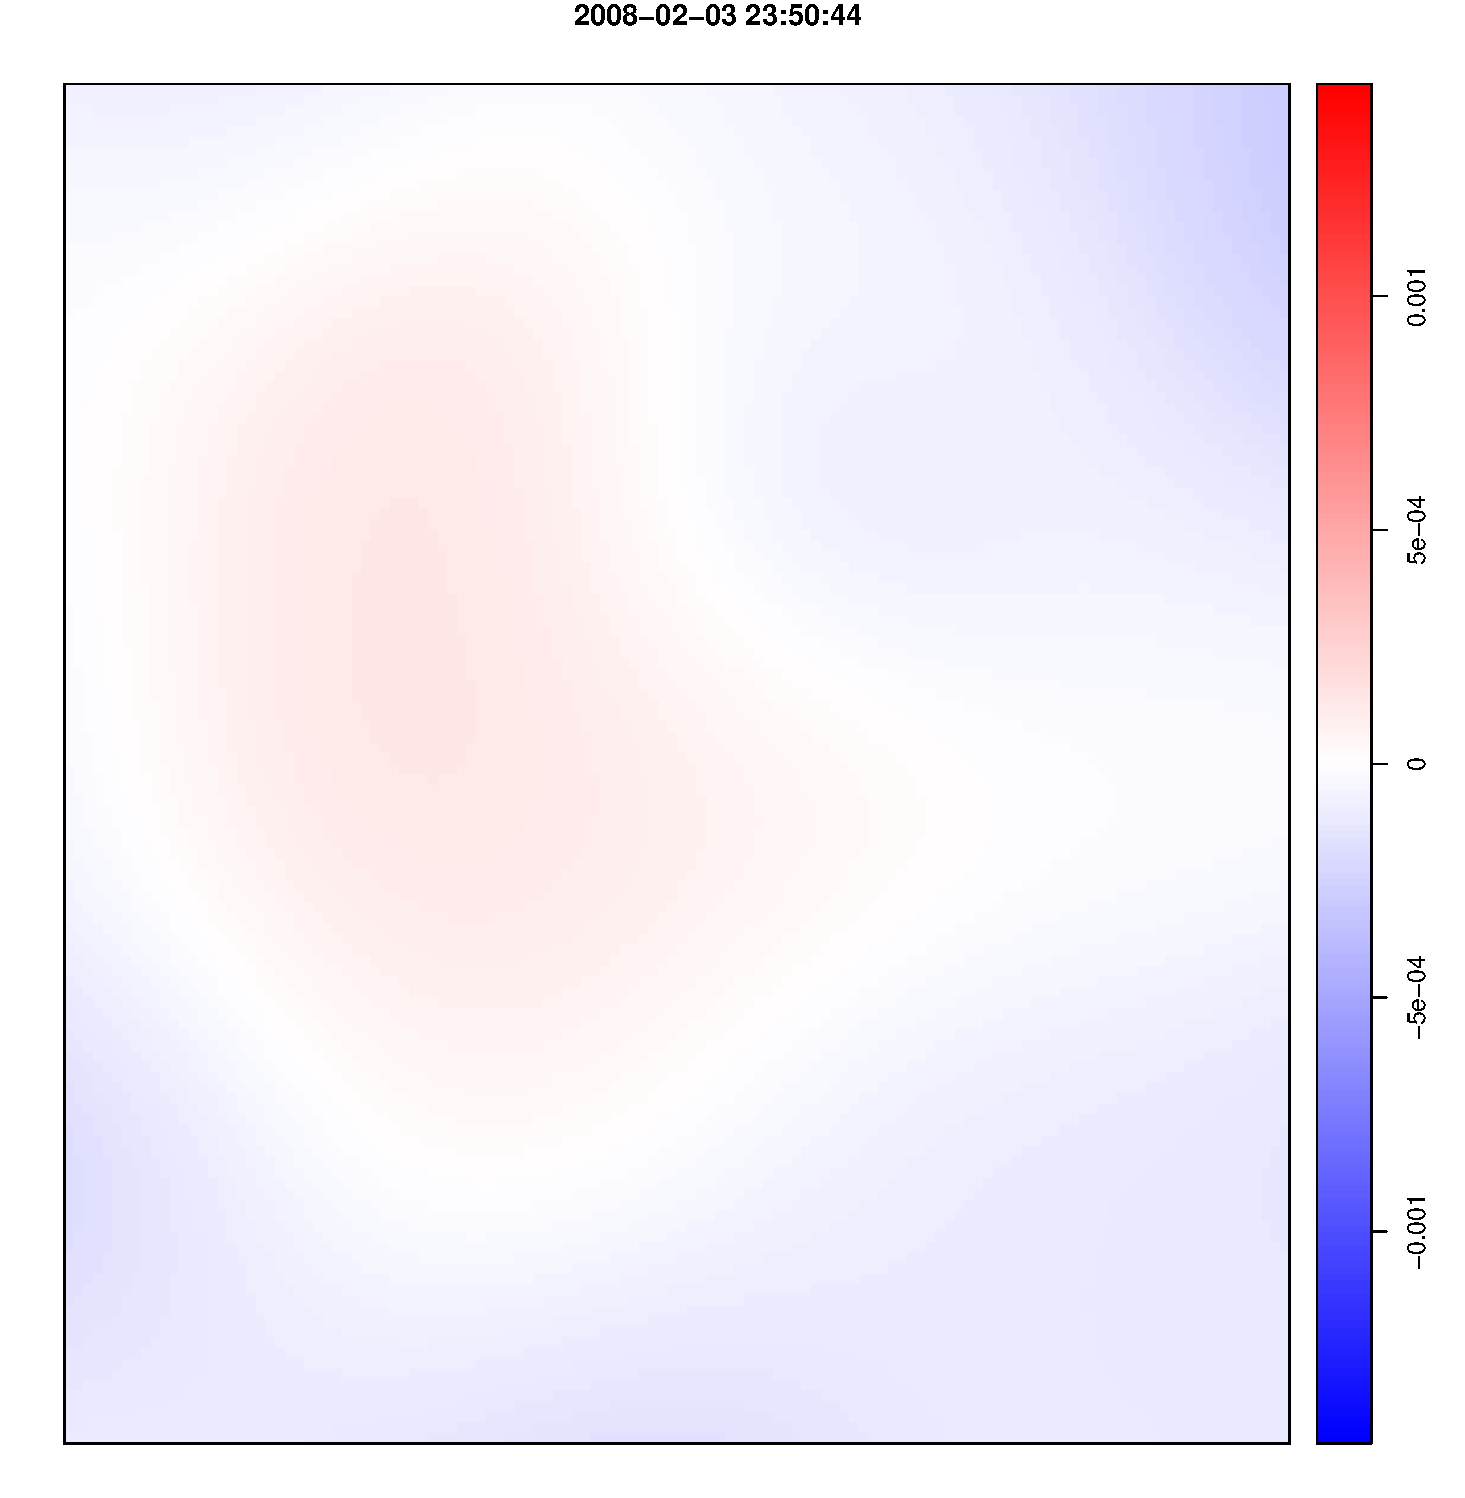
\includegraphics[width = 2.2in]{chi3}}
  \caption{Chi maps. Left: in the morning, Middle: in the afternoon, Right: at night.  Exact time is reported on each plot}
  \label{bijingchi}
  \end{figure}

\subsection{Second-order summary statistics}
  After discretising a trajectory pattern and estimating the intensity function of each single resulted point pattern, we now turn to look at the interaction between the moving objects over time. We are interested in distinguishing whether objects tend to move independently or they show some kind of dependence (e.g. clustering or inhibition). A common way in the point process literature is to use summary statistics such as $K$-function and pair correlation function \citep{ripley77,baddeley00}. Pairwise distances are the hint here: if objects tend to be close to each other, then most of the pairwise distances are going to be small, and if they favour to stand far then only a few of the pairwise distances are small \citep{BRT15}.  \cite{baddeley00} considered second-order intensity-reweighted stationary point processes, and defined the inhomogeneous $K-$function as
  \begin{eqnarray}\label{kfun}
  K_{inhom}(r) =
  \frac{1}{|B|} \ee \,
  \sum_{x_i \in B} \sum_{x_j \neq x_i} 
  \frac{\textbf{1} \{ \|x_i - x_j\| \le r \} }{ \lambda(x_i) \, \lambda(x_j)}, \hspace{1cm} r \geq 0
  \end{eqnarray}
  for any region $B \subset \R^2$ with area $|B| > 0$. The pair correlation function is given by
  \begin{eqnarray}\label{gfun}
  g(u,v)=\frac{\lambda^2(u,v)}{\lambda(u) \lambda(v)}, \qquad u,v \in W.
  \end{eqnarray}
  We point out that for Poisson point processes $K_{inhom}(r)=\pi r^2 (g(r)=1)$, and $K_{inhom}(r)>\pi r^2 (g(r)>1)$ indicates clustering, while $K_{inhom}(r)<\pi r^2 (g(r)<1)$ shows inhibition between points. There is a close relationship between the $K$-function \eqref{kfun} and the pair correlation function \eqref{gfun} as 
  \begin{eqnarray*}
  g(r)=\frac{K^{'}_{inhom}(r)}{\pi r^2}, \hspace{1cm} r>0
\end{eqnarray*}
where $K^{'}_{inhom}$ is the derivative of $K_{inhom}$.
  The plug-in estimator of the $K$-function \eqref{kfun} is of the form
  \begin{equation}\label{e:hatKinhom:plugin}
  \widehat{K}(r) =
  \frac{1}{|W|}\sum_i \sum_j 
  \frac{\textbf{1}\{d_{ij} \le r\} e(x_i,x_j,r)}{\widehat\lambda(x_i) \, \widehat\lambda(x_j)}, \hspace{1cm} r \geq 0
  \end{equation}
  where $d_{ij}$ is the distance between $x_i,x_j$ and $e(x_i,x_j,r)$ is an edge correction. For more details see \cite[Chapter 4]{MW03}; \cite{IPSS08,D13}; \citep[Chapter7]{BRT15}.

Summary statistics such as the $K$-function and the pair correlation function are used to analyse the type of interaction between points. Having this in mind, we next turn to use these functions in analysing the trajectory pattern $S$. Similar to our proposal for the intensity function and using summary statistics for point patterns, we here propose a variability area for the $K$-function and the pair correlation function as follows:
  \begin{leftbar}
  \begin{enumerate}
  \item According to regular timestamps, discretise the trajectory pattern $S$ and build the point patterns $\textbf{x}_1,\textbf{x}_2, \ldots, \textbf{x}_k$.
  \item For all the resulted point patterns $\textbf{x}_1,\textbf{x}_2, \ldots, \textbf{x}_k$, estimate the $K$-function using \eqref{kfun}.
  \item From the estimated $K$-functions $\widehat{K}_1, \widehat{K}_2,\ldots,\widehat{K}_k$, build the pointwise variability area of the $K$-function, i.e. for each value of distance argument $r$, sort $\widehat{K}_i(r)$ and then take the lowest and highest value amongst all; doing so for a sequence of $r$ results in a variability area for the $K$-function. This shows how the type of interaction between objects changes over time.
  \end{enumerate}
  \end{leftbar}

Note that, steps above can be applied to the pair correlation function as well.

In both functions above, users can take advantage of the bandwidth selection to first estimate the intensity function and then pass estimated intensities to the function \code{Kinhom} or \code{pcfinhom}. \code{default} is to not pass any estimated intensity function to \code{Kinhom} or \code{pcfinhom} in which the intensity will be estimated using the `leave-one-out' kernel smoother \citep{baddeley00,BRT15}. Different edge corrections can be also passed to \code{Kinhom.Track} and \code{pcfinhom.Track}. 
  
  
  Finally, we show the variability area of $K$-function and pair correlation function over time in Figure \ref{Kgvariation}. The left plot displays the variation of $K$-function, showing that for small distances taxis tend to have a clustering behaviour while for larger distances they favour inhibition. The right plot of the variation of the pair correlation function also confirms the same behaviour. Due to the preference of moving within particular zones, $K$-function and pair correlation function might result as what is displayed in Figure \ref{Kgvariation}. In other words, taxis might prefer to take passengers to close destinations within particular zones rather than far destinations. 
\begin{Schunk}
\begin{Sinput}
R>  # K <- Kinhom.Track(Beijing,timestamp = "20 mins",q=0)
R>  # plot(K)
R>  # g <- pcfinhom.Track(Beijing,timestamp = "20 mins",q=0)
R>  # plot(g)
\end{Sinput}
\end{Schunk}
  
  \begin{figure}[!h]
  \centering
  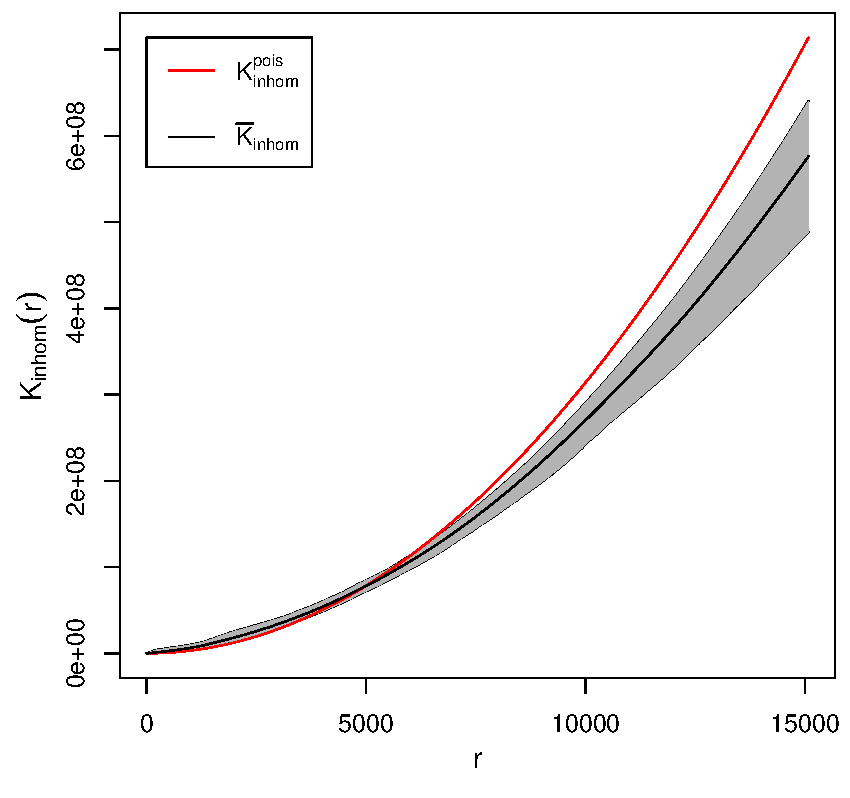
\includegraphics[width = 3in]{Kfun}
  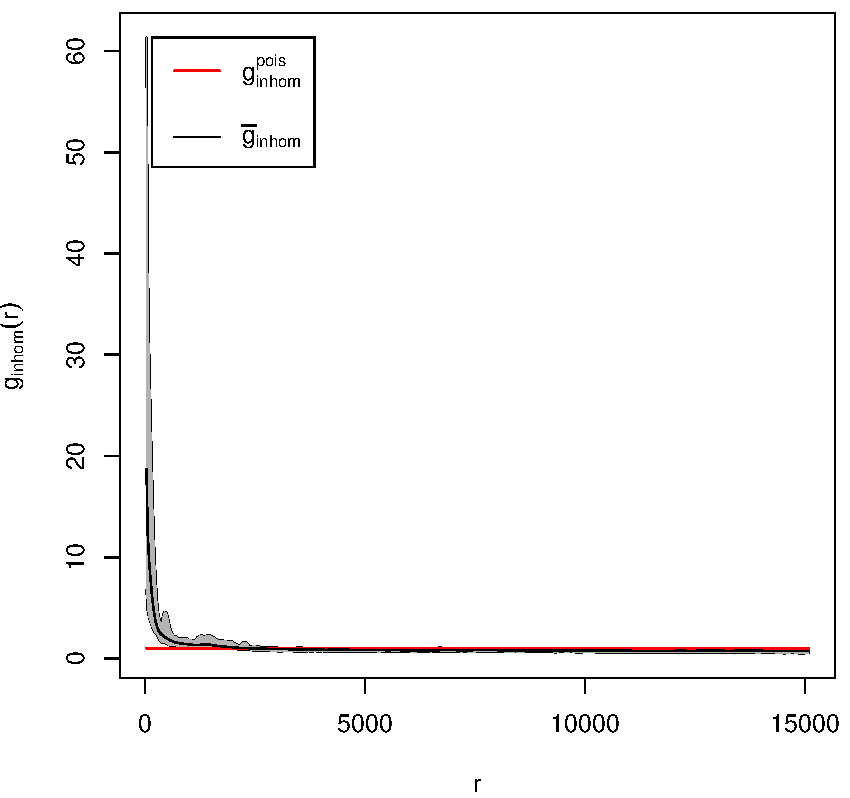
\includegraphics[width = 3in]{gfun}
  \caption{Variability area of second-order summary statistics for taxi data in Beijing, China. Left: $K$-function, Right: pair correlation function.}
  \label{Kgvariation}
  \end{figure}

  We point out that as this kind of discretising trajectory patterns results in a set of spatial point patterns, it may also drives us to consider them as replicated spatial point patterns. Therefore, one may be able to introduce a single $K$-function or pair correlation function for all patterns. For more details, see \cite[Section 5.4]{D13}.
  
 \section{Summary and discussion} \label{sec:summary}
  Analysing trajectory data is often a challenge as moving objects are living in space while moving in time. Such data might be analysed in space or time separately. However, one may look at trajectory patterns with a different perspective. 
  
  In this paper, we introduced a set of classes to handle trajectory data and defined a set of methods to summarise trajectory patterns. We have considered different classes to handle tracks passed by one object or a group of objects. We also aimed at statistically analysing trajectory data in space and see the changes in the behaviour of data over time. To do so, the literature of spatial point processes has been adapted to trajectory patterns. An average intensity function is defined for a trajectory pattern with tracks that overlap in time and it nicely reveals the more visited spots, streets, highways, etc. Pairwise distances between different objects have been also considered in \pkg{trajectories} showing how moving objects interact over time. Moreover, we have implemented methods to smooth the length of movements over time which highlights where objects move faster/slower. In addition, the discrepancy between the estimated intensity and the expected intensity per location per time can be studied in \pkg{trajectories} which shows how the mass is moving within the studied area over time. We finally presented a variability area for second-order summary statistics such as $K$-function and pair correlation function which displays the type of interaction between objects over time, highlighting possible clustering or inhibition.
  
  To perform an exploratory data analysis, we finally applied the developed methodologies to a taxi data from Beijing, China. The results nicely highlight the behaviour of taxis over time. We have recognized where the more visited spots are and also at what time data pattern is denser or objects get closer to each other. We smoothed the movements of taxis and discovered where/what time they mover faster. Not surprisingly, results confirm that moving within the city is slower than countryside or highways. Also, in the afternoon there is a decrease in the length of movements which might be affected by traffic. Chi maps have been studied showing how the mass is moving within the studied area. They display that objects are moving from countryside to the city in the morning making a heavy traffic in the city in the afternoon, as the estimated intensity is higher than the expected one. Chi maps also confirm that the  discrepancy between the estimated intensity and the expected one is less during the evening than any other time. The variability area of $K$-function and pair correlation function show that for small distances, taxis tend to show a clustering behaviour while for longer distances they show repulsion.
  
  We leave open the analysis of the effect of the environment on moving objects and the corresponding parametric analysis for future works.
  
\section*{Acknowledgments}

M.M. Moradi  gratefully acknowledges funding from the European union through the GEO-C project (H2020-MSCA-ITN-2014, Grant Agreement Number 642332, http:// www.geo-c.eu/. J. Mateu is partially funded by grants MTM2016-78917-R and P1-1B2015-40. Benedikt Klus, Benedikt Gr\"{a}ler and Nikolai Gorte are acknowledged for code contributions to the \pkg{spacetime} package.


%% -- Bibliography -------------------------------------------------------------
%% - References need to be provided in a .bib BibTeX database.
%% - All references should be made with \cite, \citet, \citep, \citealp etc.
%%   (and never hard-coded). See the FAQ for details.
%% - JSS-specific markup (\proglang, \pkg, \code) should be used in the .bib.
%% - Titles in the .bib should be in title case.
%% - DOIs should be included where available.

\bibliography{refs}


%% -- Appendix (if any) --------------------------------------------------------
%% - After the bibliography with page break.
%% - With proper section titles and _not_ just "Appendix".

%% -----------------------------------------------------------------------------


\end{document}
